\documentclass[11pt]{article}
\usepackage[margin=1in]{geometry}
\usepackage{authblk}
\usepackage{graphicx}
\usepackage{booktabs}
\usepackage{array}
\usepackage{longtable}
\usepackage{hyperref}
\usepackage{caption}
\usepackage{float}
\usepackage{amsmath}

\title{Interpretable QSAR machine-learning model for passive intestinal permeability prediction using PAMPA data and virtual screening of DrugBank compounds}

\author[1]{Benjamin Andres Vasquez Perez}
\author[1]{Juan Alberto Castillo-Garit}
\affil[1]{Facultad de Ciencias Naturales, Matematicas y del Medio Ambiente, Universidad Tecnologica Metropolitana, Santiago, Chile}
\date{}

\begin{document}
\maketitle

\section*{Abstract}
\textbf{Background:} Passive intestinal permeability is a key determinant of oral drug absorption and remains a frequent attrition factor during early drug discovery. The parallel artificial membrane permeability assay (PAMPA) provides a reproducible in vitro approximation of passive diffusion and is suitable for ligand-based computational modeling. \textbf{Methods:} A curated PAMPA dataset was assembled and divided into training, internal test and external validation sets. Molecular descriptors were calculated in alvaDesc from SMILES as 0D--2D descriptors and structural fingerprints. After alvaDesc filtering, exploratory data analysis, variance filtering, correlation analysis and Random-Forest recursive feature elimination reduced the descriptor space from 783 variables to 50 candidates. A WEKA-based consensus selection strategy then retained 11 final descriptors for a Random Forest classifier. The model was evaluated by cross-validation, internal and external validation, applicability-domain analysis, SHAP interpretation, a five-molecule prospective pre-screening set and virtual screening of DrugBank compounds. \textbf{Results:} The final model achieved accuracies of 0.863, 0.751 and 0.887 for the training, internal test and external validation sets, respectively. The corresponding AUC values were 0.940, 0.830 and 0.678, and the external validation F1-score was 0.938. The selected descriptor panel combined lipophilicity, topology, polar surface pharmacophoric information, polarizability and structural fingerprints, providing a chemically interpretable model. DrugBank screening yielded 863 high-probability candidates from a source library of more than 10000 compounds; 850 were within the applicability domain, 778 satisfied the implemented Lipinski filter and 770 satisfied both criteria. \textbf{Conclusion:} The proposed workflow provides a reproducible and interpretable QSAR model for prioritizing compounds with favorable passive intestinal permeability and can be integrated into early-stage virtual screening pipelines.

\textbf{Keywords:} PAMPA; QSAR; passive permeability; Random Forest; ADME; virtual screening; DrugBank; applicability domain.

\section{Introduction}
Low oral bioavailability remains one of the central causes of failure in drug discovery, because therapeutic activity depends not only on potency but also on the ability of a compound to reach the systemic circulation at suitable concentrations \cite{DiMasi2016,Kola2004}. In this context, absorption, distribution, metabolism and excretion (ADME) properties are increasingly evaluated during the early design stage instead of being deferred to late development \cite{Lipinski2001,Siramshetty2021}. Intestinal permeability is especially relevant for orally administered drugs, and the distinction between passive diffusion and transporter-mediated processes is important when selecting experimental and computational endpoints \cite{Lennernas2007,Jorgensen2025}.

The parallel artificial membrane permeability assay (PAMPA) is a high-throughput experimental method designed to estimate passive membrane permeation using an artificial lipid barrier \cite{Kansy1998,Sugano2001}. Compared with cellular systems such as Caco-2 or MDCK, PAMPA does not include active transporters, metabolic enzymes or paracellular complexity. However, this narrower biological scope can be advantageous for machine-learning benchmarking, because the endpoint is more directly related to physicochemical and structural features of the molecule \cite{Sun2017}. For QSAR modeling, a well-defined PAMPA endpoint therefore provides a consistent basis for learning the relationship between molecular structure and passive permeability.

Quantitative structure-activity/property relationship (QSAR/QSPR) models are based on the premise that molecular structure encodes the information needed to estimate physicochemical or biological behavior \cite{Todeschini2000}. Modern machine-learning algorithms extend classical linear QSAR by capturing nonlinear patterns and interactions among descriptors. Random Forests are particularly useful in this setting because they are robust to descriptor interactions, provide internal measures of variable importance and can be combined with interpretability analyses \cite{Breiman2001,Lundberg2017}. Previous studies have shown the utility of machine-learning QSAR in ADME prediction and virtual screening \cite{CastilloGarit2008,Sun2017,CasanolaMartin2018,Barigye2021,CanizaresCarmenate2022,Parasar2025}.

For a QSAR model to be scientifically defensible, it should follow the OECD principles: a defined endpoint, an unambiguous algorithm, a defined applicability domain, appropriate measures of goodness of fit and predictivity, and mechanistic interpretation when possible \cite{OECD2007}. The present work follows these principles by developing a reproducible, interpretable Random Forest classifier for PAMPA permeability prediction. The model was validated using internal and external datasets, a prospective five-molecule pre-screening set, and a virtual screening workflow applied to DrugBank compounds.

\section{Materials and Methods}
\subsection{Dataset curation and endpoint definition}
The modeling dataset was compiled from compounds with experimentally reported PAMPA permeability classes. The curated data were organized into three sets: a training set of 4357 compounds, an internal test set of 1090 compounds and an independent external validation set of 486 compounds. The binary endpoint was encoded as permeable (\texttt{Act1}) or non-permeable (\texttt{Act-1}). Table~\ref{tab:datasets} summarizes the final class distribution, and Figure~\ref{fig:py_dataset_distribution} visualizes the same split to make the class imbalance easier to inspect. The external dataset was not used during model training or feature selection, preserving its role as an independent generalization test.

\begin{table}[H]
\centering
\caption{Dataset composition used for model development and validation.}
\label{tab:datasets}
\begin{tabular}{lrrr}
\toprule
Dataset & Total compounds & Permeable & Non-permeable \\
\midrule
Training & 4357 & 2332 & 2025 \\
Internal test & 1090 & 583 & 507 \\
External validation & 486 & 443 & 43 \\
\bottomrule
\end{tabular}
\end{table}

\begin{figure}[H]
\centering
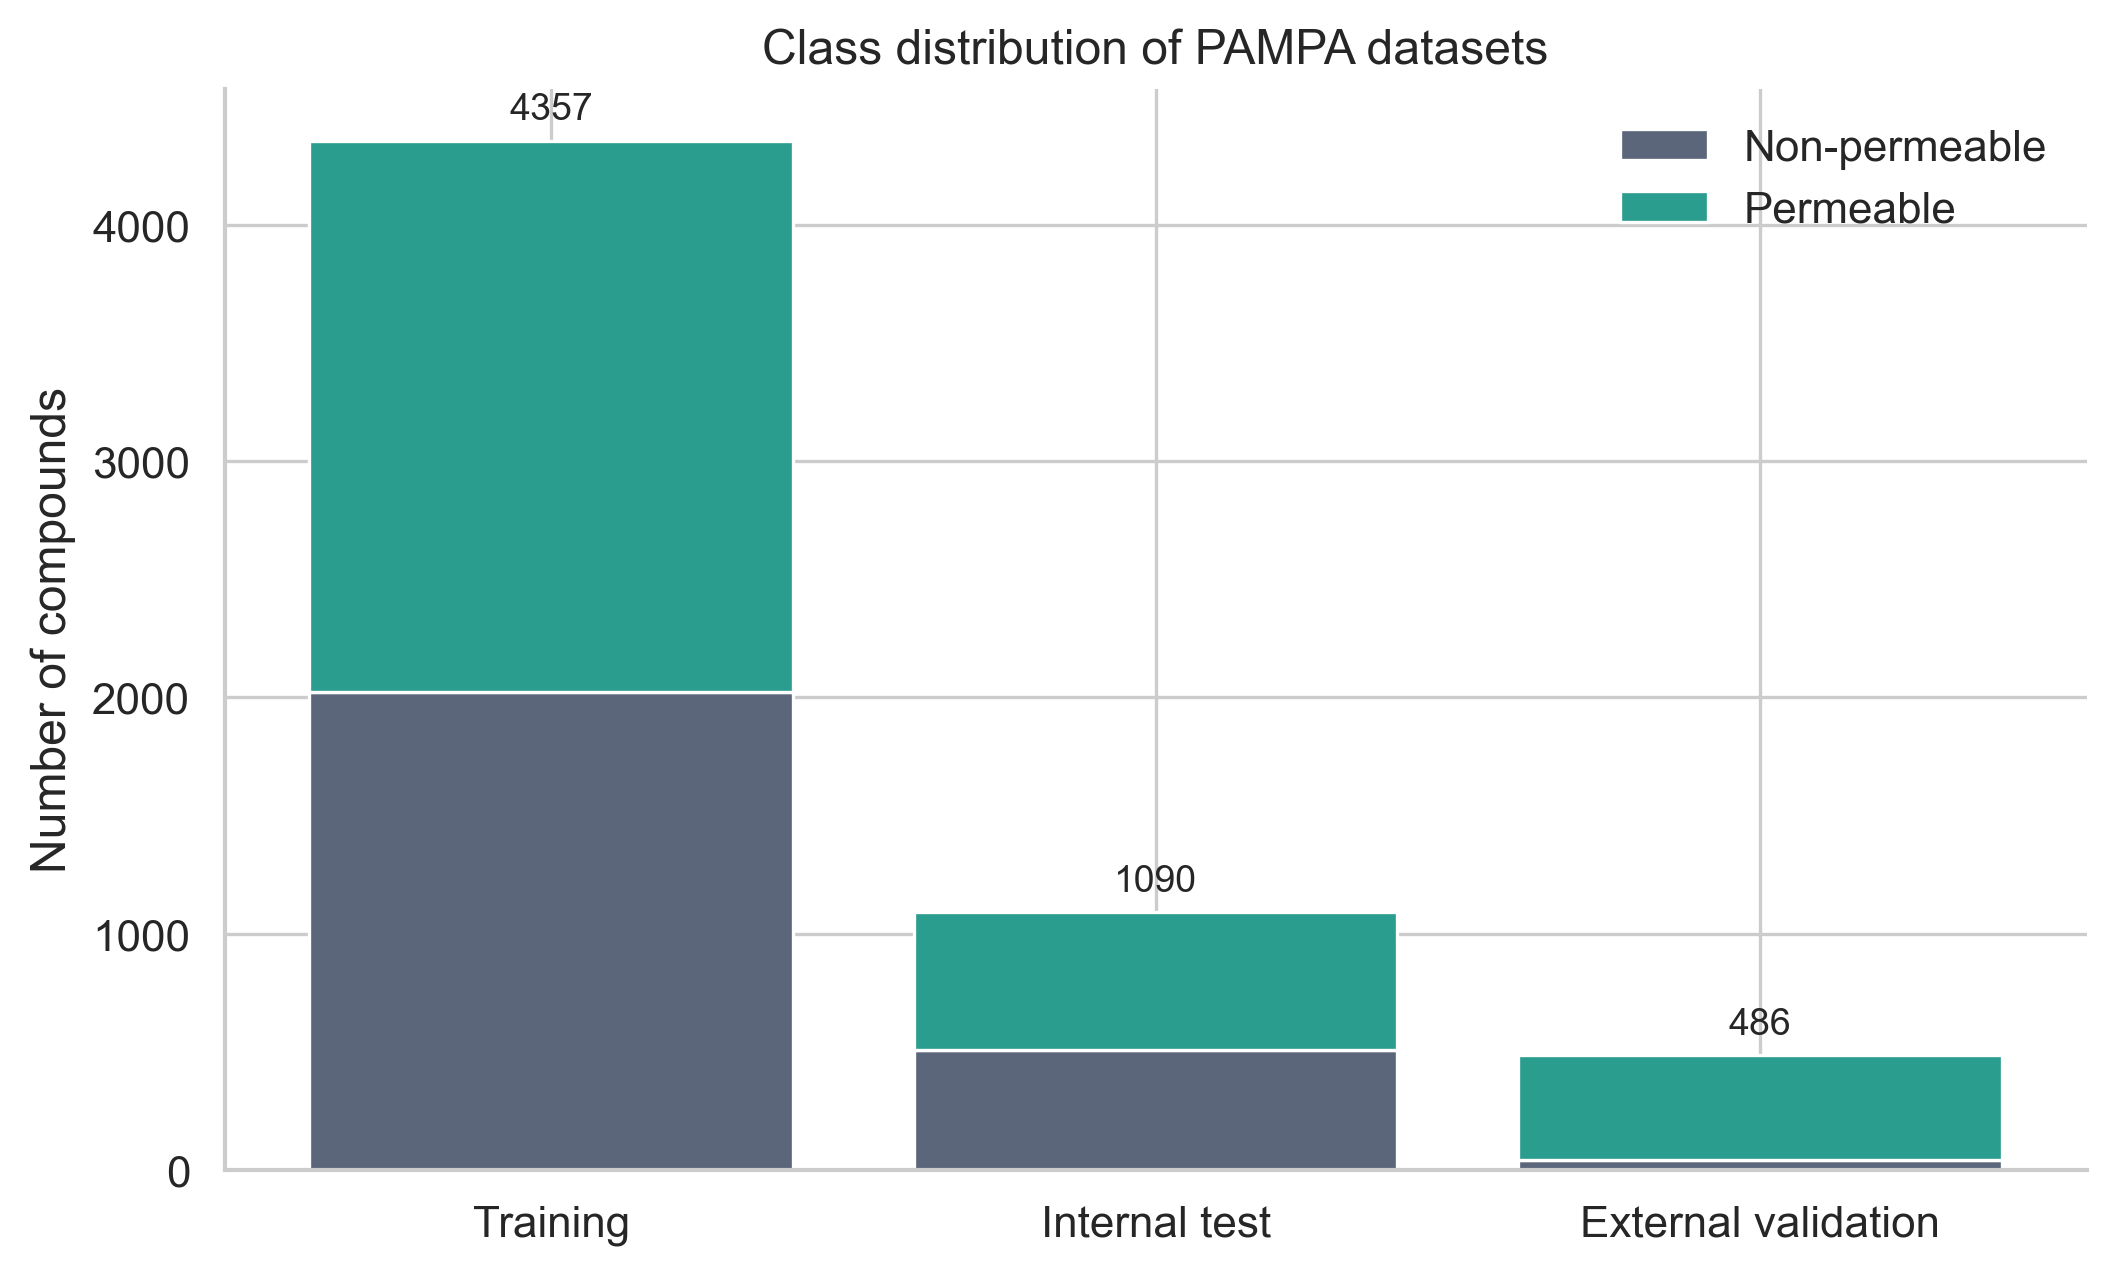
\includegraphics[width=0.78\textwidth]{figures/python_dataset_class_distribution.png}
\caption{Python-generated class distribution of the curated PAMPA datasets.}
\label{fig:py_dataset_distribution}
\end{figure}

\subsection{Molecular representation with alvaDesc}
The curated structures were standardized as SMILES before descriptor calculation. Molecular descriptors were calculated with alvaDesc v.2.0.10. Because the workflow started from SMILES and was intended to remain compatible with large-scale virtual screening, only 0D--2D descriptors were retained together with structural fingerprints, including MACCS and ECFP-type fingerprints. This first molecular representation encoded constitutional, topological, electronic, physicochemical and substructural information for each compound.

The raw descriptor matrix was reduced inside alvaDesc by removing descriptors with constant or near-constant values and descriptors with pairwise correlation above 85\%. This initial software-level filter removed variables that could not contribute meaningful discrimination or that were redundant before any model-dependent selection. The filtered matrix still contained 783 descriptors, which was too high-dimensional for a stable and interpretable QSAR classifier.

\subsection{Exploratory data analysis and preselection}
Before WEKA consensus selection, an exploratory data analysis (EDA) stage was performed in Python to evaluate data integrity and descriptor behavior. Missing and infinite values were checked, descriptor types were verified and the class distribution was inspected. The training set showed a moderate predominance of permeable compounds, while the external validation set was strongly enriched in permeable compounds; therefore, model assessment emphasized sensitivity, specificity, F1-score, MCC and AUC rather than accuracy alone.

EDA was also used as a dimensionality-reduction step. Low-variance descriptors were removed using a variance threshold of 0.05, because descriptors with almost no dispersion across compounds were unlikely to discriminate permeable from non-permeable molecules. Pearson and Spearman correlation analyses were then used to identify families of highly collinear descriptors, especially among topological and constitutional variables. Mann--Whitney comparisons between permeability classes were used diagnostically to highlight descriptors with class-dependent distributions. Finally, Random-Forest recursive feature elimination (RFE), based on preliminary Gini importance, reduced the 783-descriptor matrix by approximately 90\%, yielding an intermediate set of 50 descriptors for the WEKA selection stage. This preselection lowered computational cost while preserving chemically informative variables for consensus voting.

\subsection{WEKA-based consensus feature selection}
A Python automation layer was used to run WEKA attribute-selection procedures. The maintained implementation in this repository is \texttt{src/weka\_feature\_selection.py}, which replaces the historical exploratory script \texttt{weka\_cmd1.py}. Ten selector combinations were generated by pairing two classifiers, J48 and IBk, with five search strategies: BestFirst, GeneticSearch, LinearForwardSelection, RankSearch and SubsetSizeForwardSelection. Descriptor votes were obtained from the selected-attribute logs. A preliminary vote threshold of 40\% identified candidate variables; a subsequent parsimony step retained the 11 descriptors that maximized predictive performance without reducing model stability.

Operationally, \texttt{weka\_cmd1.py} served as the original orchestration script that launched all WEKA selector configurations and collected the selected-attribute outputs. In the reproducible repository, the same logic is separated into explicit commands for generating WEKA calls, running the selectors and summarizing descriptor votes. The voting stage treated each selector as one independent evaluator, so descriptors selected by at least four of the ten runs entered the parsimony review. This design avoided dependence on a single selection algorithm and made the final 11-descriptor panel a consensus result rather than the product of one ranking method.

\subsection{Model training}
The final model was a \texttt{RandomForestClassifier} implemented in scikit-learn \cite{Pedregosa2011}. The saved model uses 500 trees, maximum depth of 10, minimum leaf size of 4, square-root feature sampling, class weights of 1.5 for the non-permeable class and 1.0 for the permeable class, and a fixed random seed of 42. The model was trained on a balanced representation of the training data while preserving the original datasets for final evaluation.

\subsection{Validation strategy}
Model performance was assessed using a hierarchical validation strategy: cross-validation on the training data, evaluation on the original training set, evaluation on the internal test set, and evaluation on the external validation set. Accuracy, sensitivity, specificity, area under the receiver operating characteristic curve (AUC), Matthews correlation coefficient (MCC) and F1-score were calculated. The final metrics can be reproduced with:

\begin{verbatim}
python src/check_final_metrics.py
\end{verbatim}

The applicability domain was estimated using leverage. For a descriptor matrix \(X\), the leverage of a compound was calculated from the diagonal of:

\[
H = X(X^TX)^{-1}X^T
\]

The warning leverage threshold was defined as \(h^* = 3(p+1)/n\), where \(p\) is the number of descriptors and \(n\) is the number of training compounds.

\subsection{Prospective pre-screening and DrugBank virtual screening}
The model was first challenged with five molecules not used for training, corresponding to the prospective pre-screening step described in the thesis and associated with recently reported multitarget compounds \cite{Waheed2026}. This set contained three 4-hydrazono-pyrazolidinedione derivatives reported as compounds 2, 3 and 7, plus Donepezil as a positive PAMPA control and Norfloxacin as a negative PAMPA control. The exercise was qualitative because the reported experimental values corresponded to PAMPA-BBB, whereas the model endpoint was intestinal passive permeability; however, both assays probe passive diffusion through an artificial membrane.

A larger virtual screening workflow was then applied to DrugBank-derived compounds \cite{Wishart2018}. The complete DrugBank source contained more than 10000 entries before descriptor availability, curation and filtering. The screening was implemented as a funnel: descriptor calculation and model prediction, probability filtering at \(P(\mathrm{permeable}) \geq 0.60\), applicability-domain filtering by leverage with \(h^* = 0.0083\), and Lipinski-like drug-likeness filtering. Final candidate tables were interpreted as prioritization lists rather than definitive pharmacokinetic annotations.

\section{Results and Discussion}
\subsection{Consensus-selected descriptors}
The final model retained 11 descriptors (Table~\ref{tab:descriptors}). The panel is chemically coherent for passive permeability because it combines lipophilicity, aromatic/heteroatom fingerprints, topology, polarizability, donor surface terms and descriptors related to electronic distribution. This is consistent with the expected balance between membrane affinity and desolvation cost during passive diffusion.

\begin{longtable}{p{0.22\textwidth}p{0.23\textwidth}p{0.45\textwidth}}
\caption{Final descriptors used by the Random Forest PAMPA model.}
\label{tab:descriptors}\\
\toprule
Descriptor & Descriptor family & Mechanistic interpretation \\
\midrule
\endfirsthead
\toprule
Descriptor & Descriptor family & Mechanistic interpretation \\
\midrule
\endhead
LOGPcons & Physicochemical & Consensus lipophilicity; controls affinity for the lipid-like membrane phase. \\
MACCSFP125 & Structural fingerprint & Encodes a heteroatom-containing aromatic pattern that may capture favorable two-dimensional pharmacophoric features. \\
PCR & Topological & Ratio of multiple path counts to simple path counts; captures molecular complexity and branching. \\
Psi\_e\_A & Electrotopological & Describes intrinsic-state pseudoconnectivity weighted by electronegativity, reflecting electronic accessibility. \\
P\_VSA\_ppp\_D & Surface/pharmacophore & Van der Waals surface associated with donor pharmacophoric points; related to desolvation cost. \\
Mp & Atomic property & Mean atomic polarizability; describes deformability of the electron cloud and dispersion interactions. \\
SpMin1\_Bh(p) & Burden matrix & Smallest eigenvalue of a Burden matrix weighted by polarizability; maps polarizable topological regions. \\
SHED\_AL & Shannon entropy & Acceptor-lipophilic distribution descriptor; captures spatial balance between polar and apolar regions. \\
SM12\_AEA(ri) & Spectral moment & Resonance-integral-weighted augmented edge adjacency moment; reflects conjugation and aromaticity. \\
P\_VSA\_s\_3 & Surface descriptor & Surface contribution associated with defined physicochemical bins. \\
MATS5m & 2D autocorrelation & Moran autocorrelation weighted by atomic mass at lag 5; captures mass distribution along molecular topology. \\
\bottomrule
\end{longtable}

\subsection{Cross-validation and final predictive performance}
Cross-validation showed stable results for 5-fold and 10-fold partitions, with AUC values of 0.823 and 0.823, respectively (Table~\ref{tab:cv}). These values indicate that the balanced training procedure did not rely on a single favorable data split.

\begin{table}[H]
\centering
\caption{Cross-validation performance of the final Random Forest model.}
\label{tab:cv}
\begin{tabular}{rrrrrr}
\toprule
K & Accuracy & Sensitivity & Specificity & AUC & F1-score \\
\midrule
5 & 0.738 & 0.729 & 0.746 & 0.823 & 0.735 \\
10 & 0.738 & 0.730 & 0.745 & 0.823 & 0.735 \\
\bottomrule
\end{tabular}
\end{table}

The final model reproduced the thesis metrics on the training, internal test and external validation sets (Table~\ref{tab:metrics}). The heatmap in Figure~\ref{fig:py_metric_heatmap} summarizes these metrics across validation levels, while the confusion matrices in Figure~\ref{fig:py_confusion_matrices} show the distribution of correct and incorrect class assignments. The ROC curves in Figure~\ref{fig:roc} provide the discrimination profile of the model, and Figure~\ref{fig:importance} shows the Random Forest variable-importance ranking. The training AUC of 0.940 and test AUC of 0.830 indicate good discrimination within the main chemical space. In the external validation set, the model maintained high accuracy and sensitivity, with an F1-score of 0.938. The external AUC was lower (0.678), which should be interpreted in the context of strong class imbalance in the external set (443 permeable and 43 non-permeable compounds). Even under this imbalance, the model retained useful capacity for identifying permeable compounds while preserving an explicit applicability-domain filter.

\begin{table}[H]
\centering
\caption{Final model performance reproduced from the serialized model.}
\label{tab:metrics}
\begin{tabular}{lrrrrrr}
\toprule
Dataset & Accuracy & Sensitivity & Specificity & AUC & MCC & F1-score \\
\midrule
Training & 0.863 & 0.852 & 0.877 & 0.940 & 0.727 & 0.870 \\
Internal test & 0.751 & 0.760 & 0.742 & 0.830 & 0.501 & 0.766 \\
External validation & 0.887 & 0.939 & 0.349 & 0.678 & 0.291 & 0.938 \\
\bottomrule
\end{tabular}
\end{table}

\begin{figure}[H]
\centering
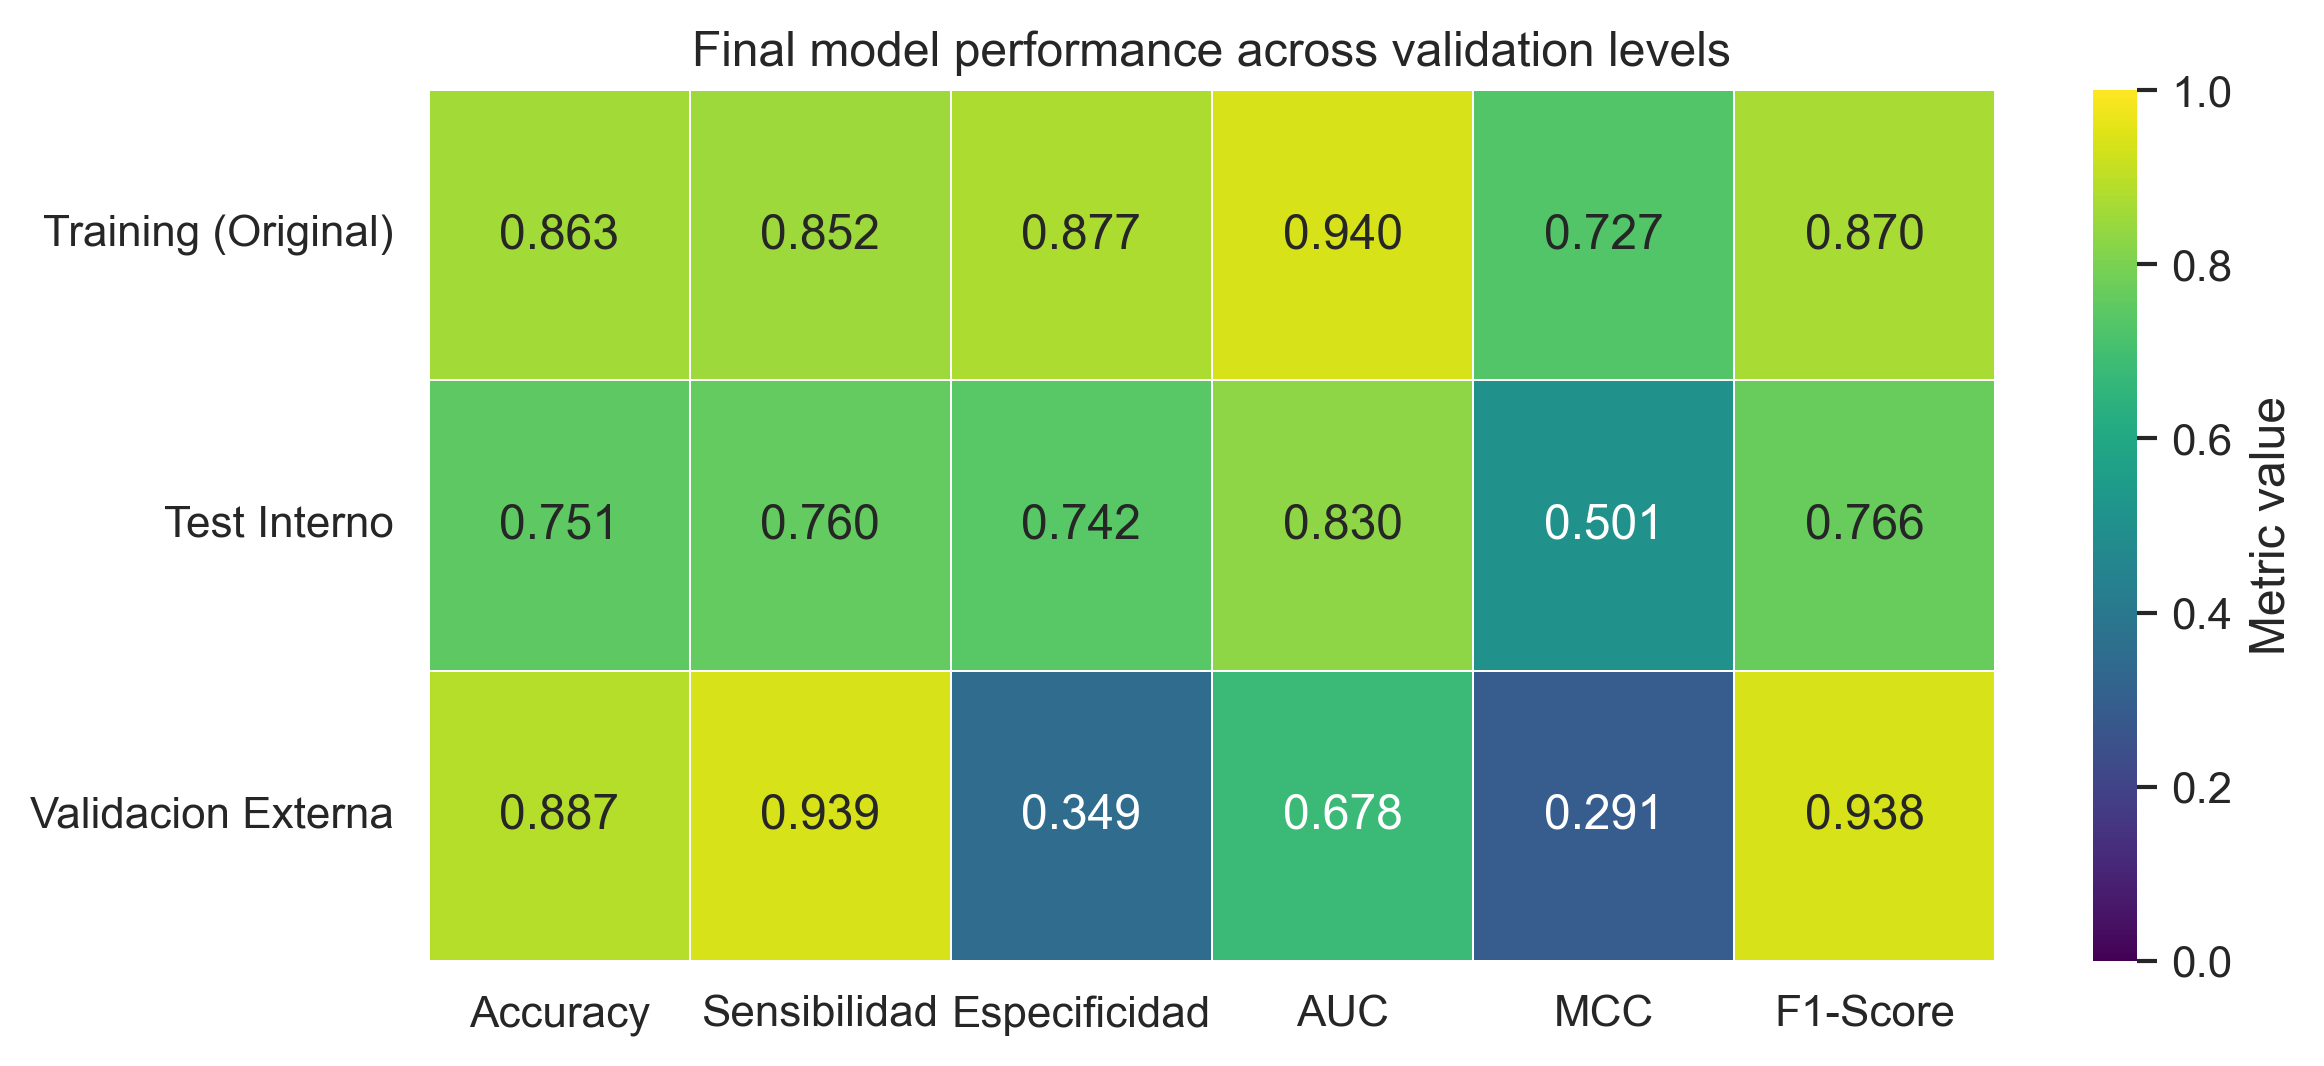
\includegraphics[width=0.86\textwidth]{figures/python_final_metrics_heatmap.png}
\caption{Python-generated heatmap of final model metrics across validation levels.}
\label{fig:py_metric_heatmap}
\end{figure}

\begin{figure}[H]
\centering
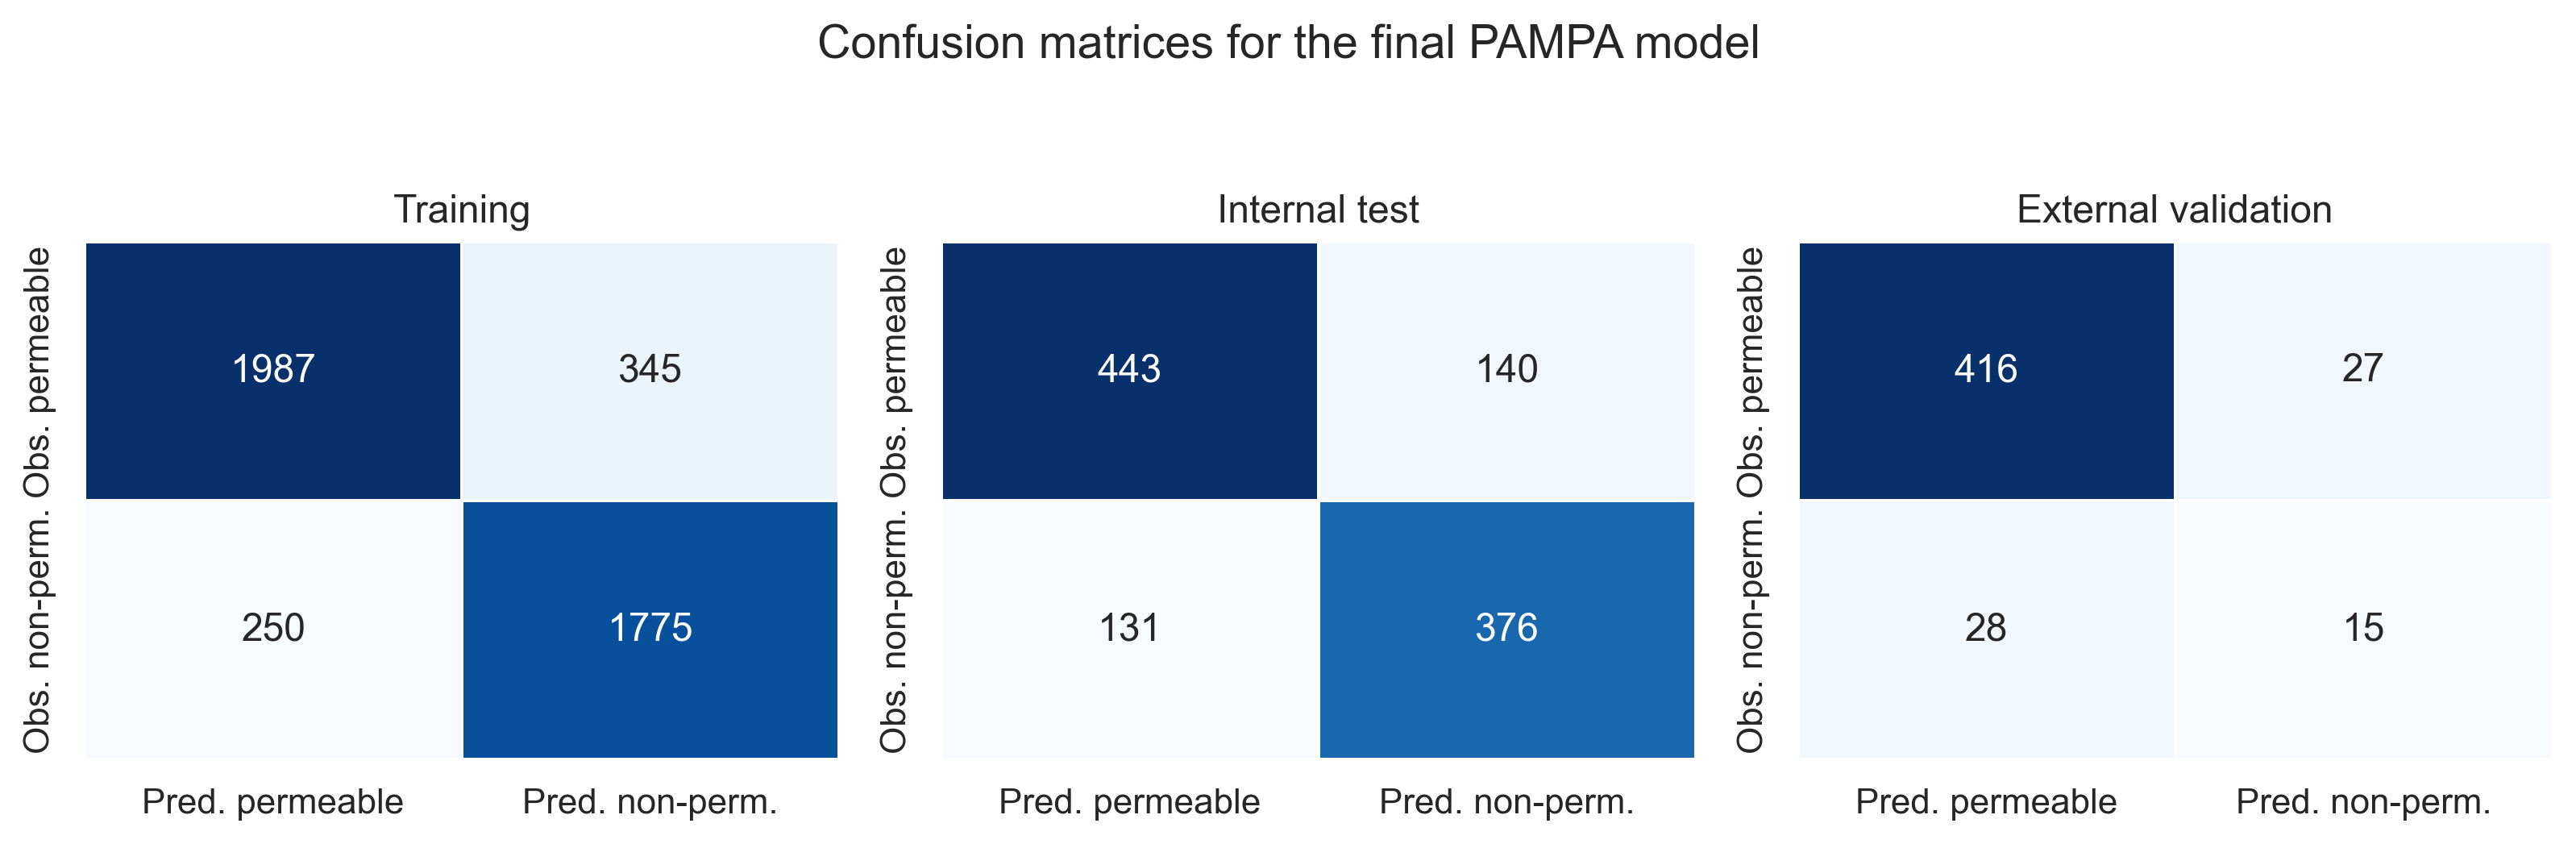
\includegraphics[width=0.95\textwidth]{figures/python_confusion_matrices.png}
\caption{Python-generated confusion matrices for the training, internal test and external validation sets. Rows correspond to observed classes and columns to predicted classes.}
\label{fig:py_confusion_matrices}
\end{figure}

\begin{figure}[H]
\centering
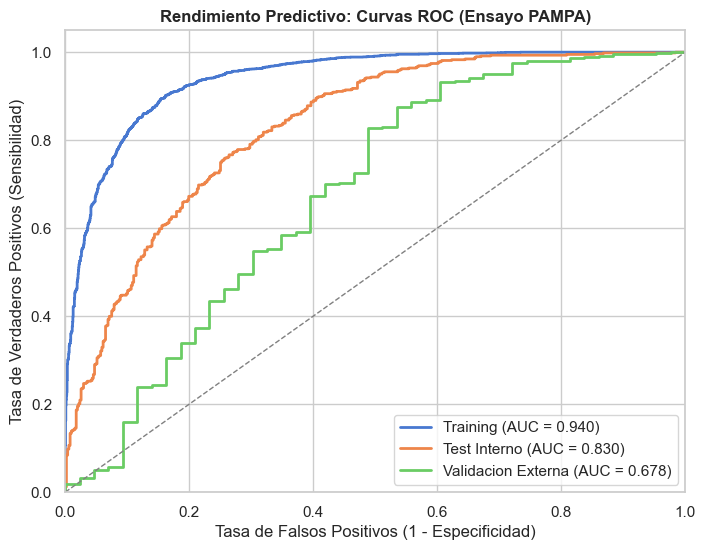
\includegraphics[width=0.85\textwidth]{figures/Curvas_ROC_PAMPA.png}
\caption{Receiver operating characteristic curves for the final PAMPA permeability model.}
\label{fig:roc}
\end{figure}

\begin{figure}[H]
\centering
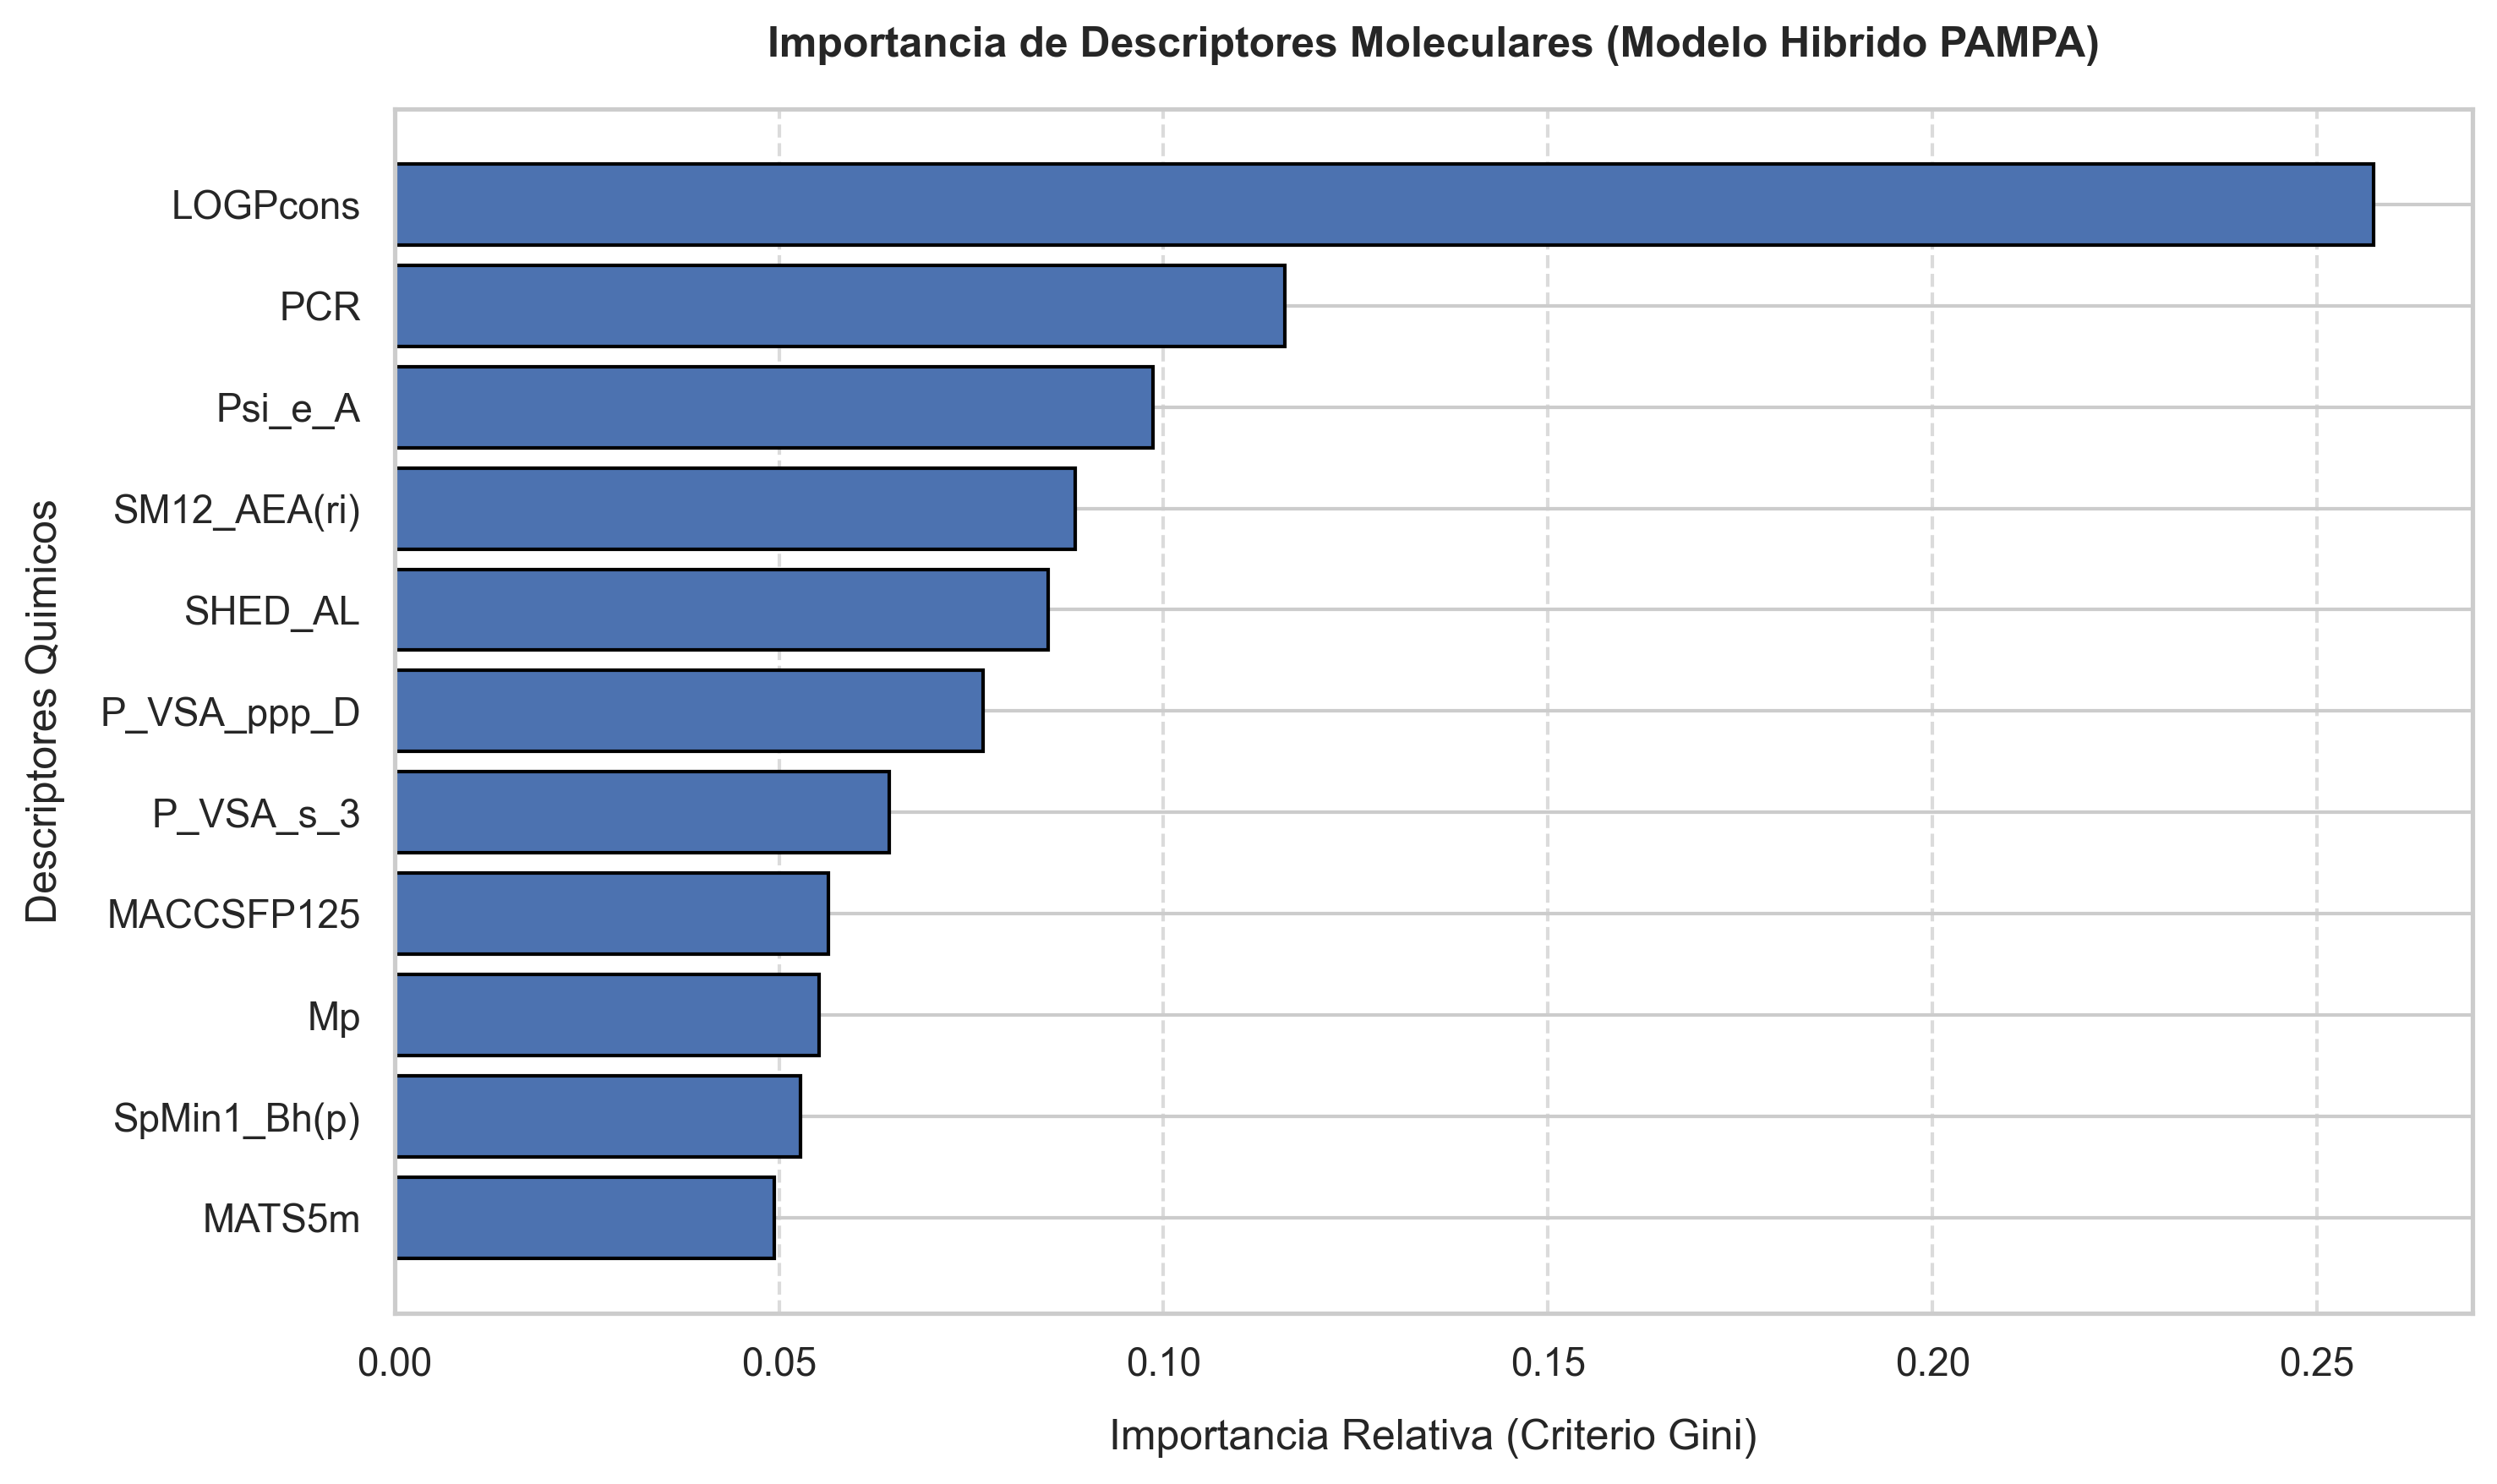
\includegraphics[width=0.85\textwidth]{figures/Importancia_Variables_PAMPA.png}
\caption{Variable-importance profile of the selected Random Forest model.}
\label{fig:importance}
\end{figure}

\subsection{SHAP-based interpretation}
In addition to Random Forest impurity-based importance, SHAP values were used as a model-agnostic interpretation layer to estimate how each descriptor contributed to the probability assigned to individual compounds \cite{Lundberg2017}. The SHAP bar plot in Figure~\ref{fig:shap_bar} summarizes mean absolute contributions across the analyzed dataset, while the beeswarm plot in Figure~\ref{fig:shap_beeswarm} preserves the directionality and dispersion of descriptor effects. This complementary analysis is useful because impurity-based importance ranks variables globally but does not show whether high or low descriptor values tend to push predictions toward the permeable class.

\begin{figure}[H]
\centering
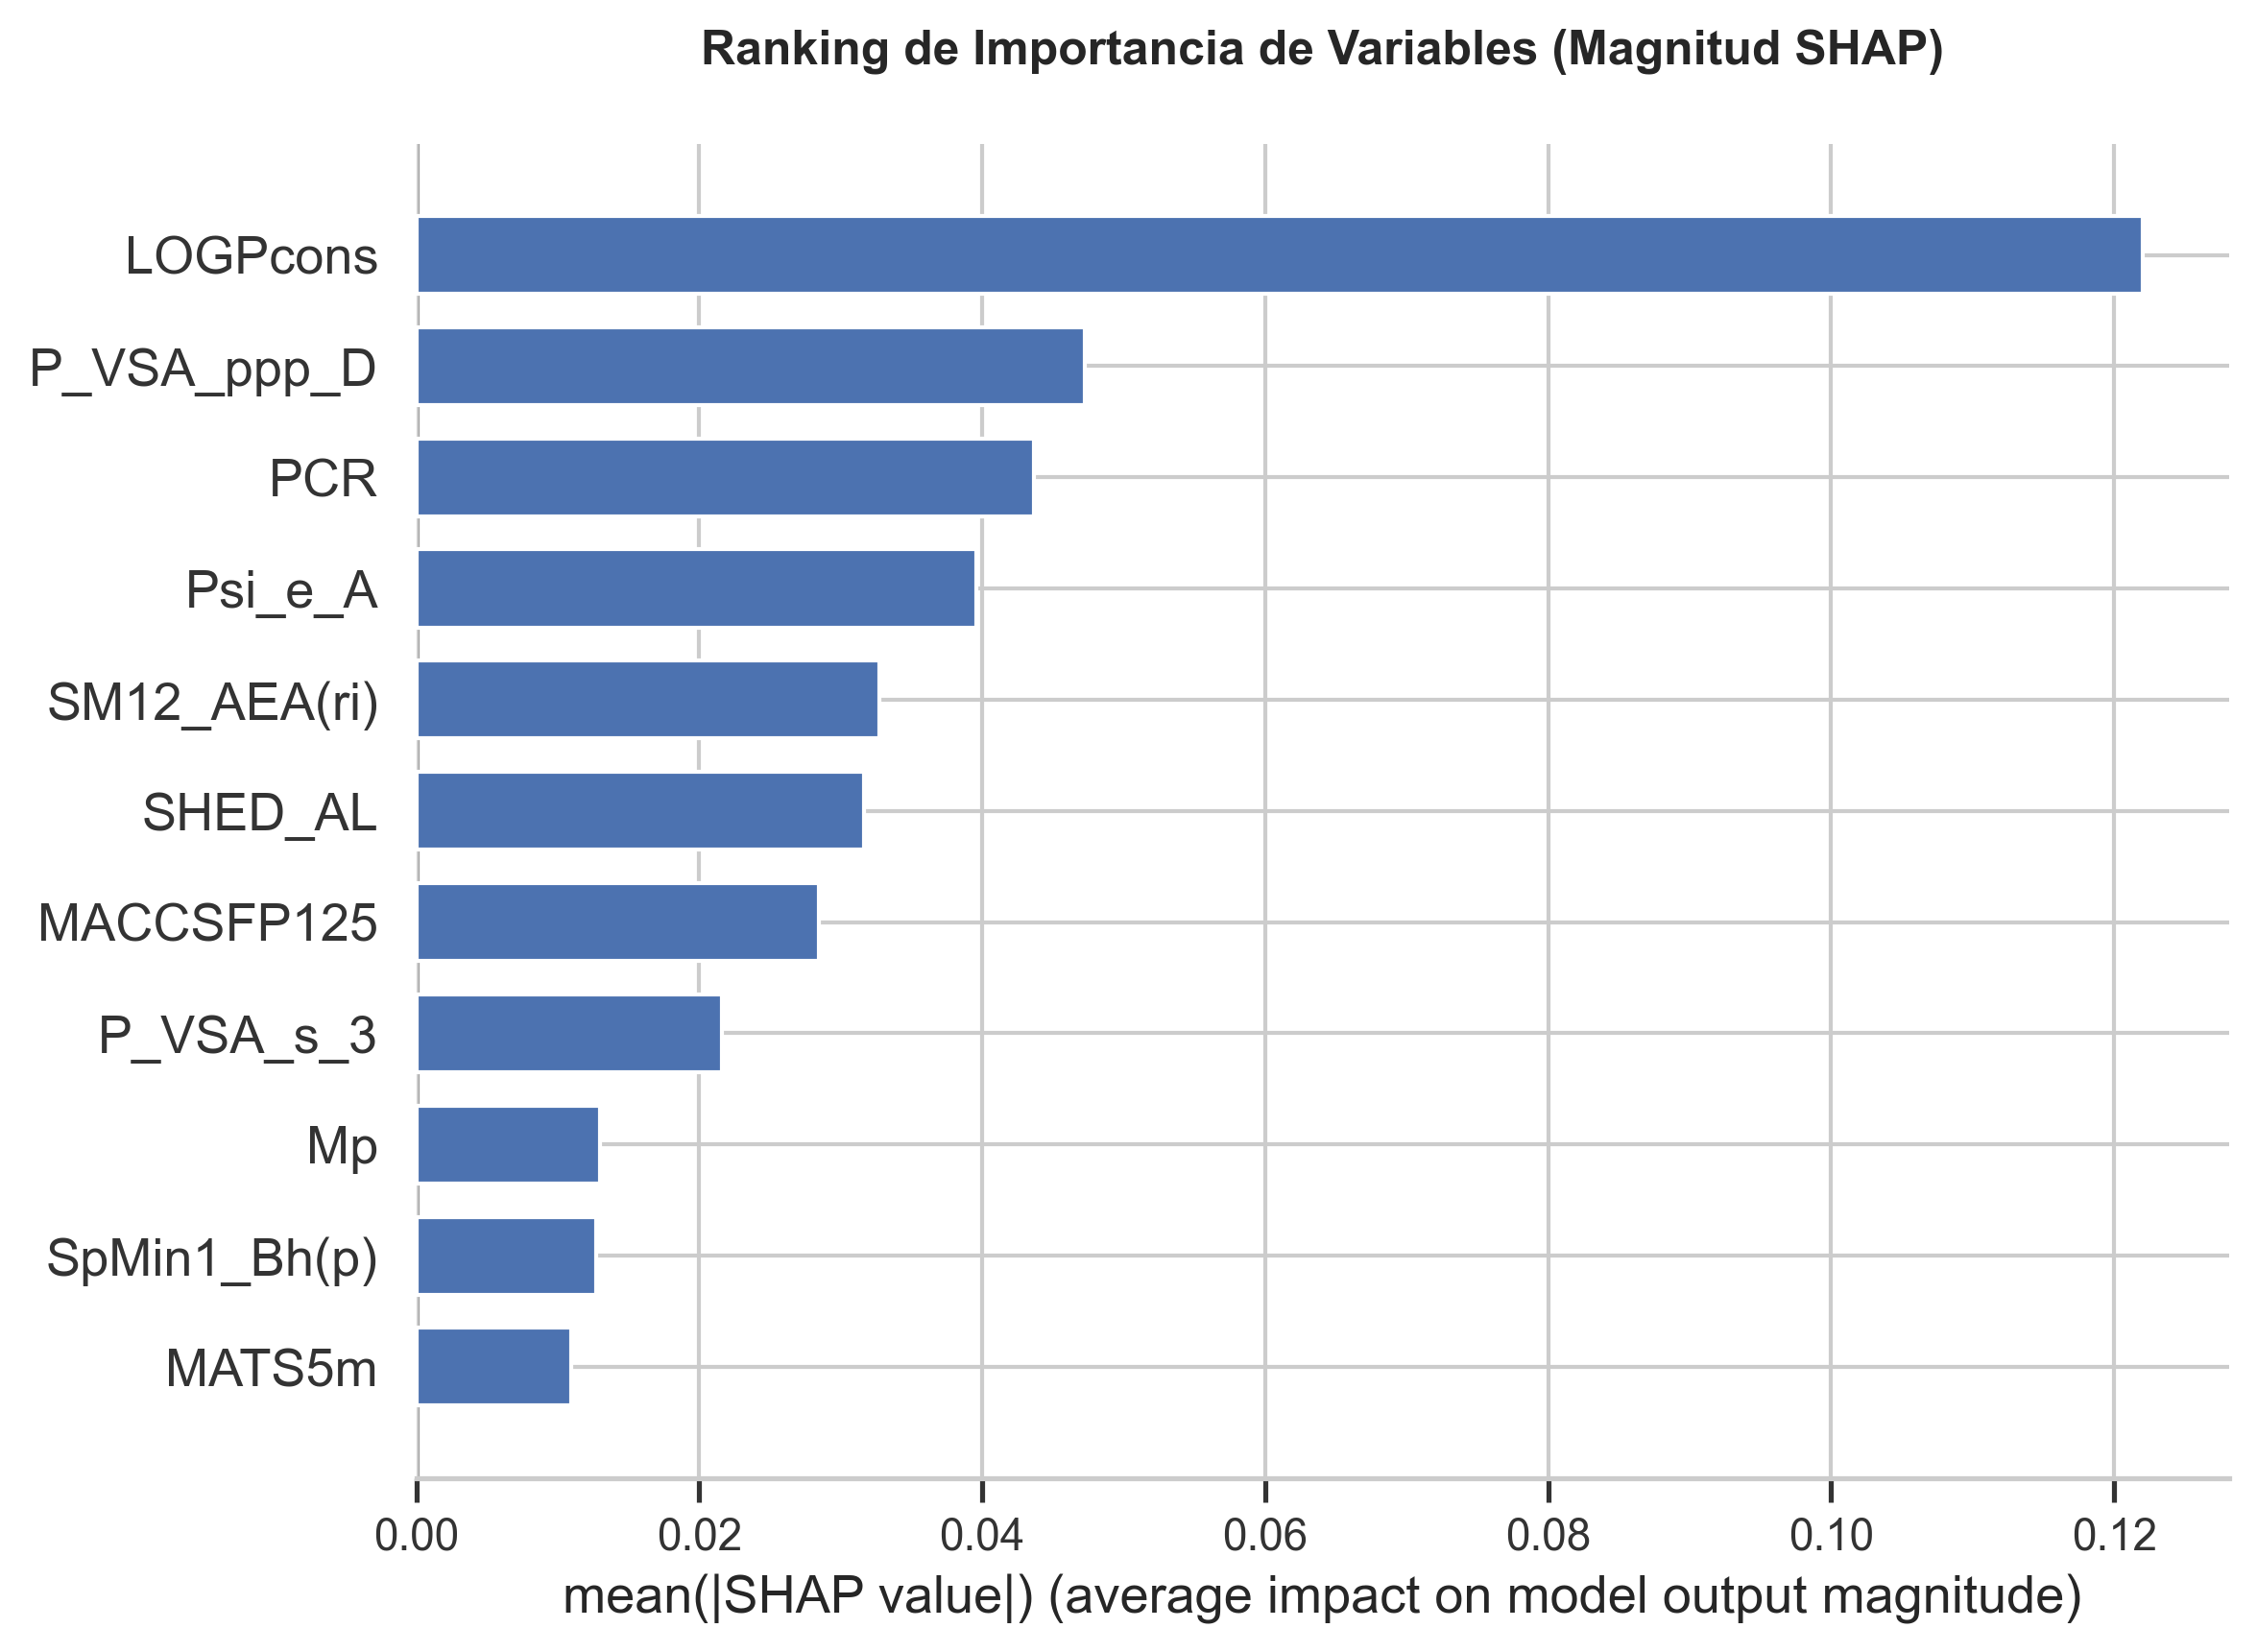
\includegraphics[width=0.82\textwidth]{figures/SHAP_Bar_PAMPA.png}
\caption{SHAP global-importance summary for the final 11-descriptor Random Forest PAMPA model.}
\label{fig:shap_bar}
\end{figure}

\begin{figure}[H]
\centering
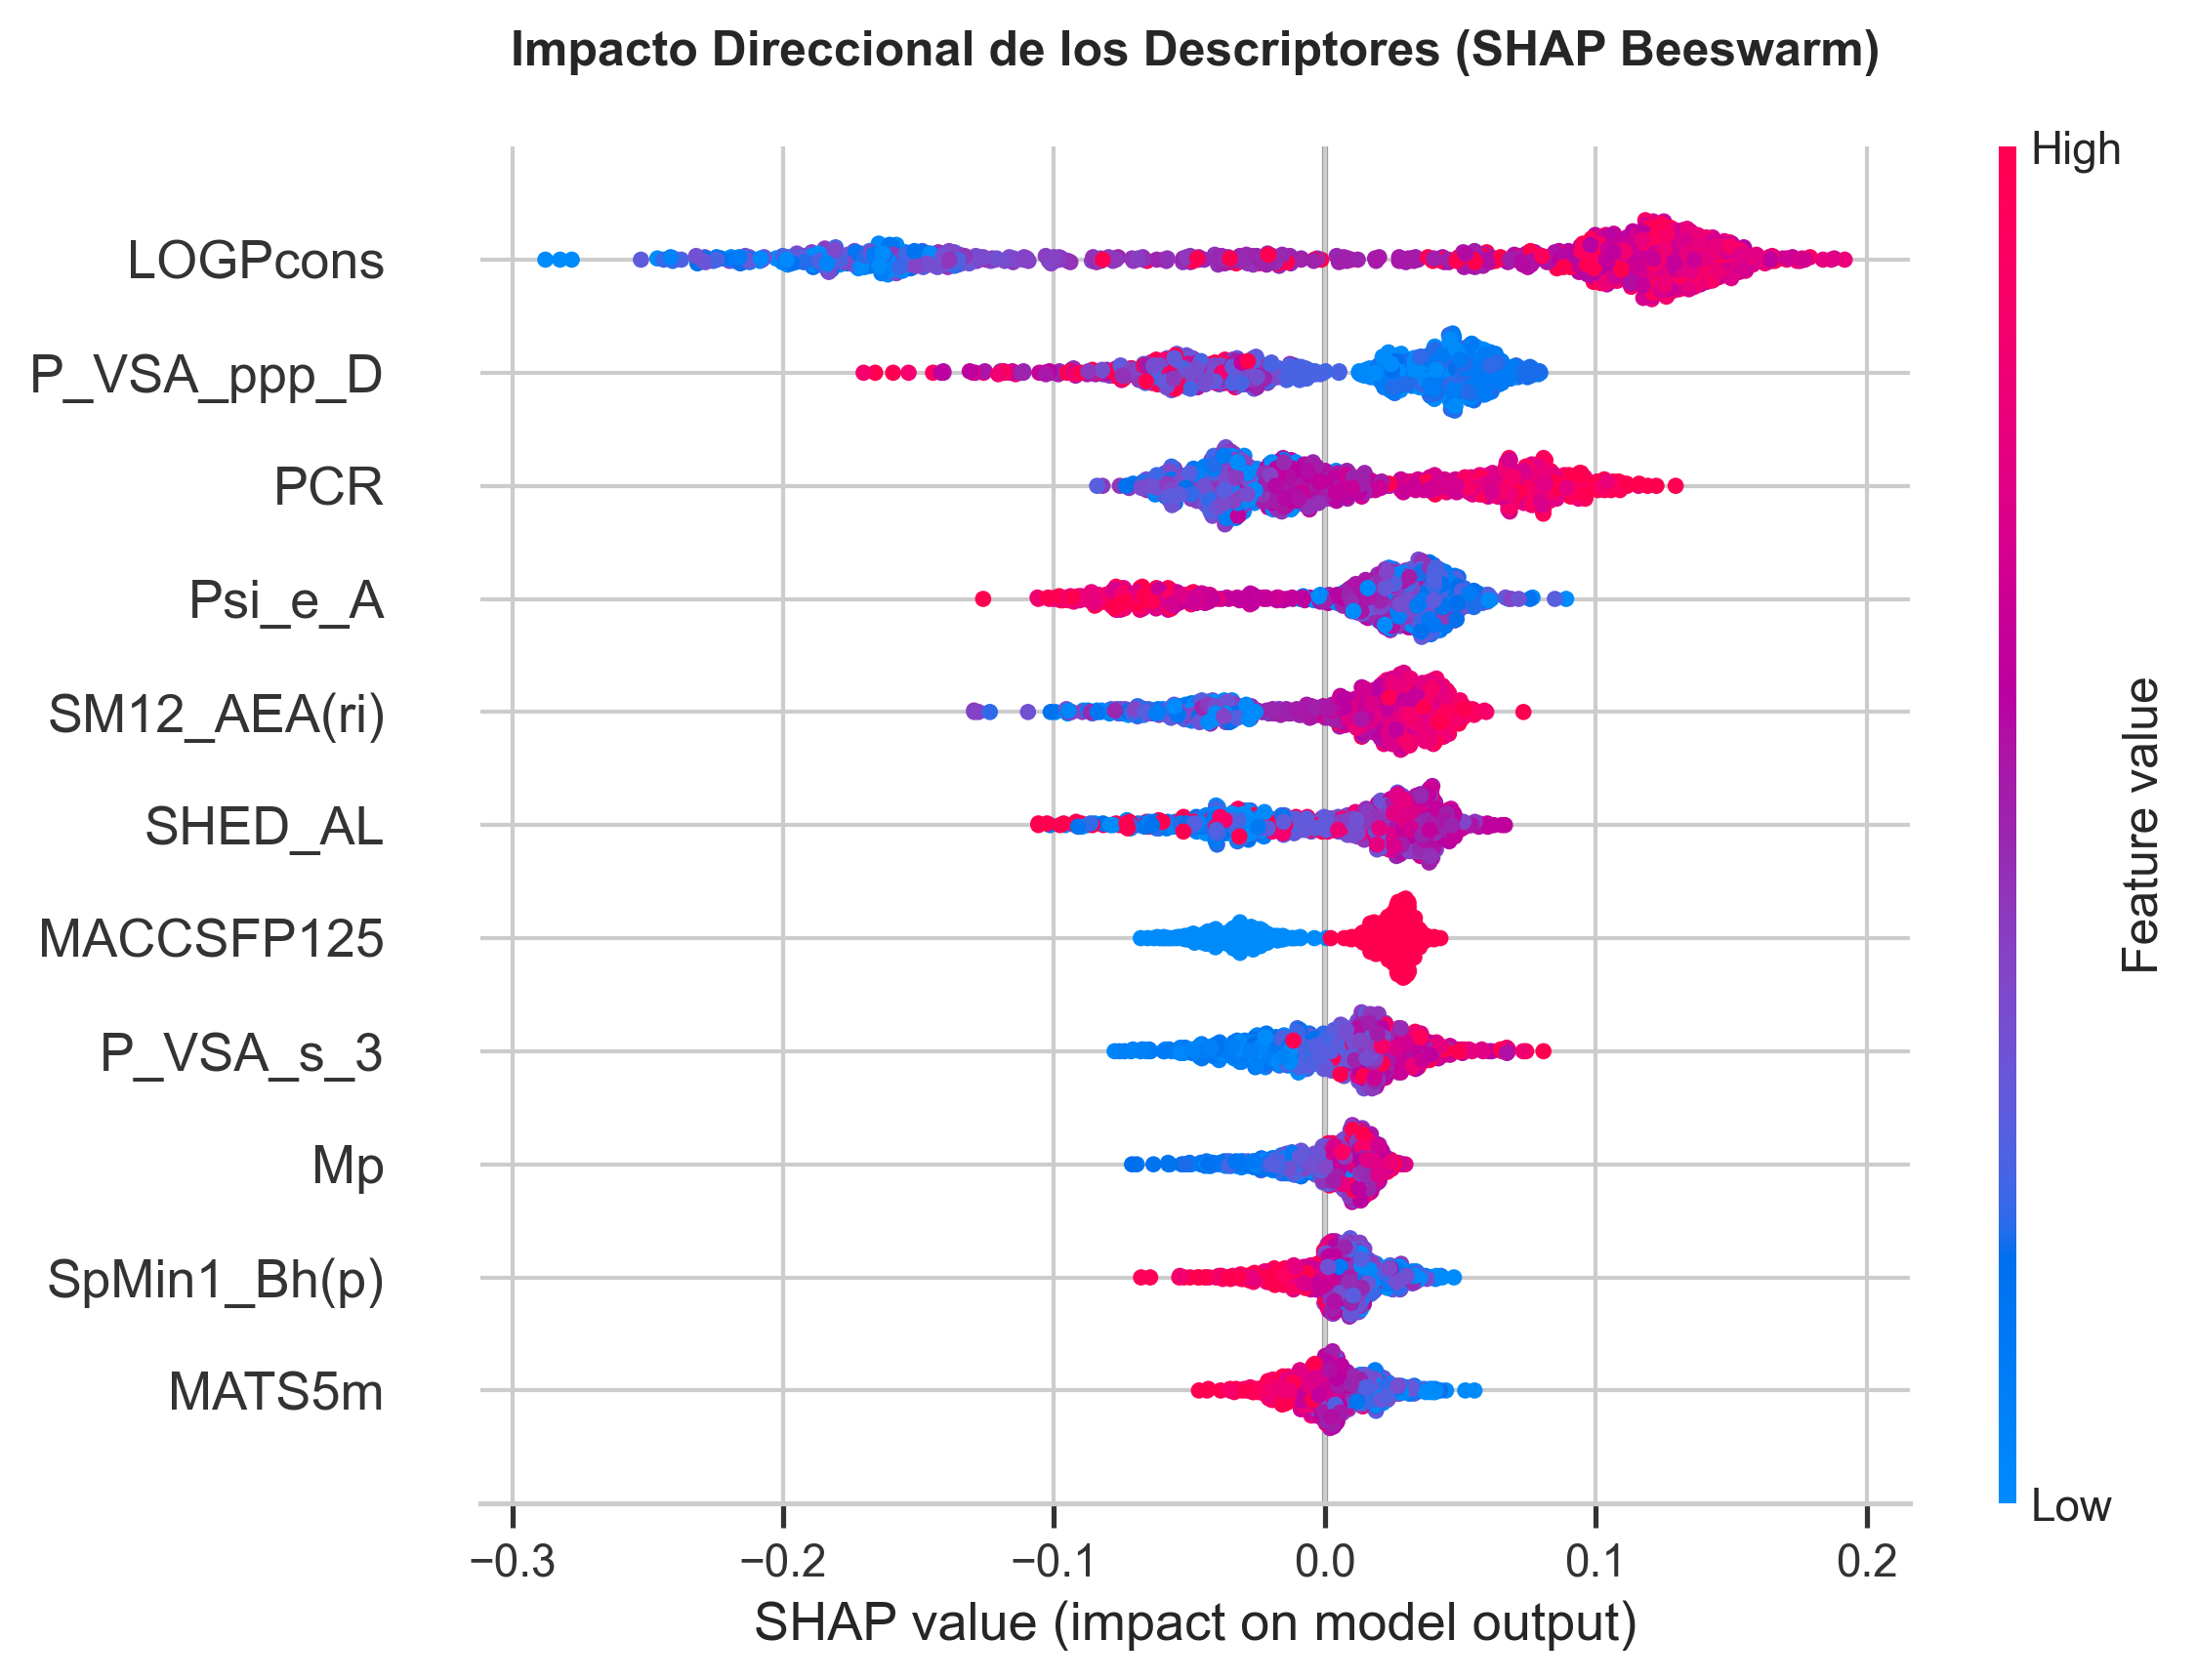
\includegraphics[width=0.86\textwidth]{figures/SHAP_Beeswarm_PAMPA.png}
\caption{SHAP beeswarm plot showing descriptor-level contributions to permeability predictions.}
\label{fig:shap_beeswarm}
\end{figure}

\subsection{Mechanistic interpretation}
The selected descriptors support a mechanistically plausible interpretation of passive permeability. LOGPcons reflects the hydrophobic contribution required for entry into the membrane phase. Donor-related surface terms, such as P\_VSA\_ppp\_D, represent polar interactions that may increase desolvation penalties before membrane partitioning. Polarizability descriptors (Mp and SpMin1\_Bh(p)) encode the capacity for induced-dipole and dispersion interactions with lipid chains. Topological and spectral descriptors (PCR and SM12\_AEA(ri)) contribute information on branching, conjugation and aromaticity, which can influence molecular shape and membrane accommodation. The inclusion of MACCSFP125 suggests that the model also benefits from a discrete structural motif associated with heteroatom-containing aromatic systems. Taken together, the Random Forest importance and SHAP summaries indicate that the final model is not driven by a single descriptor, but by a combination of lipophilicity, topology, polar surface and polarizability terms.

\subsection{Prospective pre-screening}
The five-molecule pre-screening experiment was used as a small prospective control because these compounds were not used during training. The set comprised the three selected Waheed derivatives (compounds 2, 3 and 7), Donepezil as a permeable control and Norfloxacin as a low-permeability control. Four compounds were predicted as permeable with probabilities between 0.648 and 0.696, while Norfloxacin was assigned a low permeability probability of 0.045 (Table~\ref{tab:py_prescreening_named}). The structures and experimental PAMPA values are shown in Figure~\ref{fig:py_prescreening_structures}, and the model probabilities are visualized in Figure~\ref{fig:py_prescreening}. This behavior agrees qualitatively with the experimental PAMPA values reported in the thesis table and supports the ability of the model to classify unseen structures in a chemically meaningful range. The size of this prospective set is small, so it is best interpreted as a transferability check rather than a substitute for the larger external validation.

\input{tables/pre_screening_named.tex}

\begin{figure}[H]
\centering
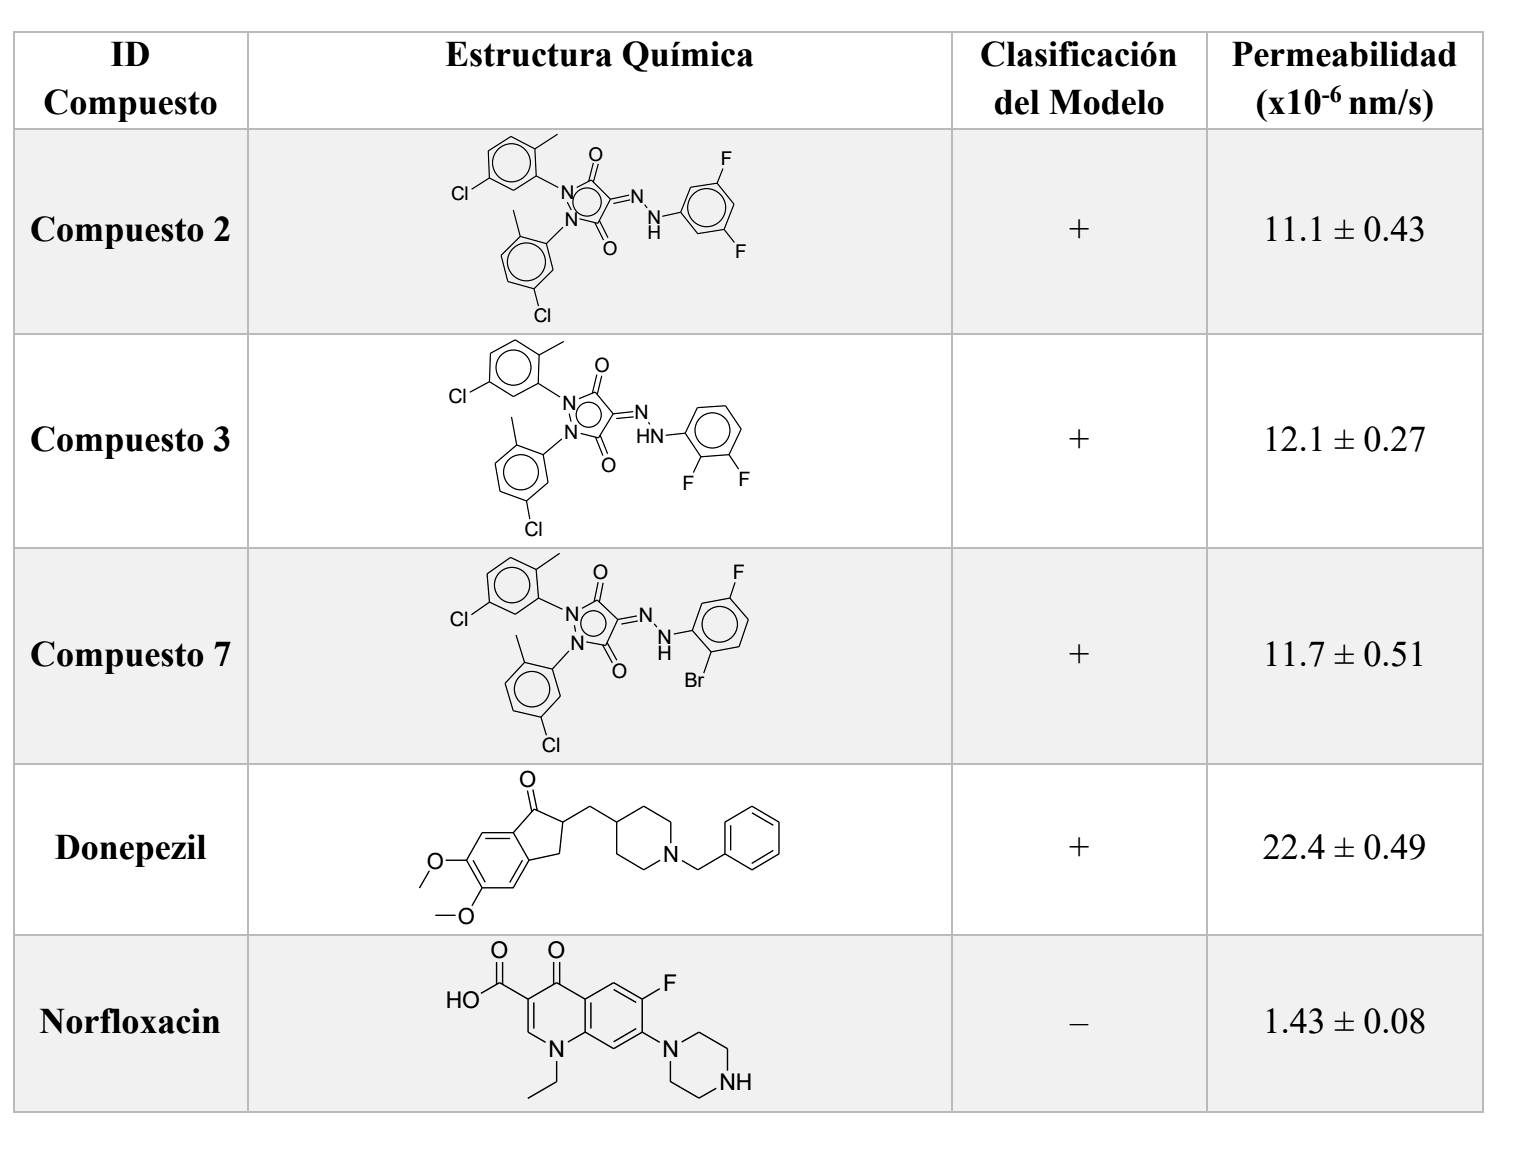
\includegraphics[width=0.95\textwidth]{figures/python_pre_screening_structures.png}
\caption{Structures and experimental PAMPA values for the five compounds used in the prospective pre-screening exercise, reproduced from the thesis table for manuscript traceability.}
\label{fig:py_prescreening_structures}
\end{figure}

\begin{figure}[H]
\centering
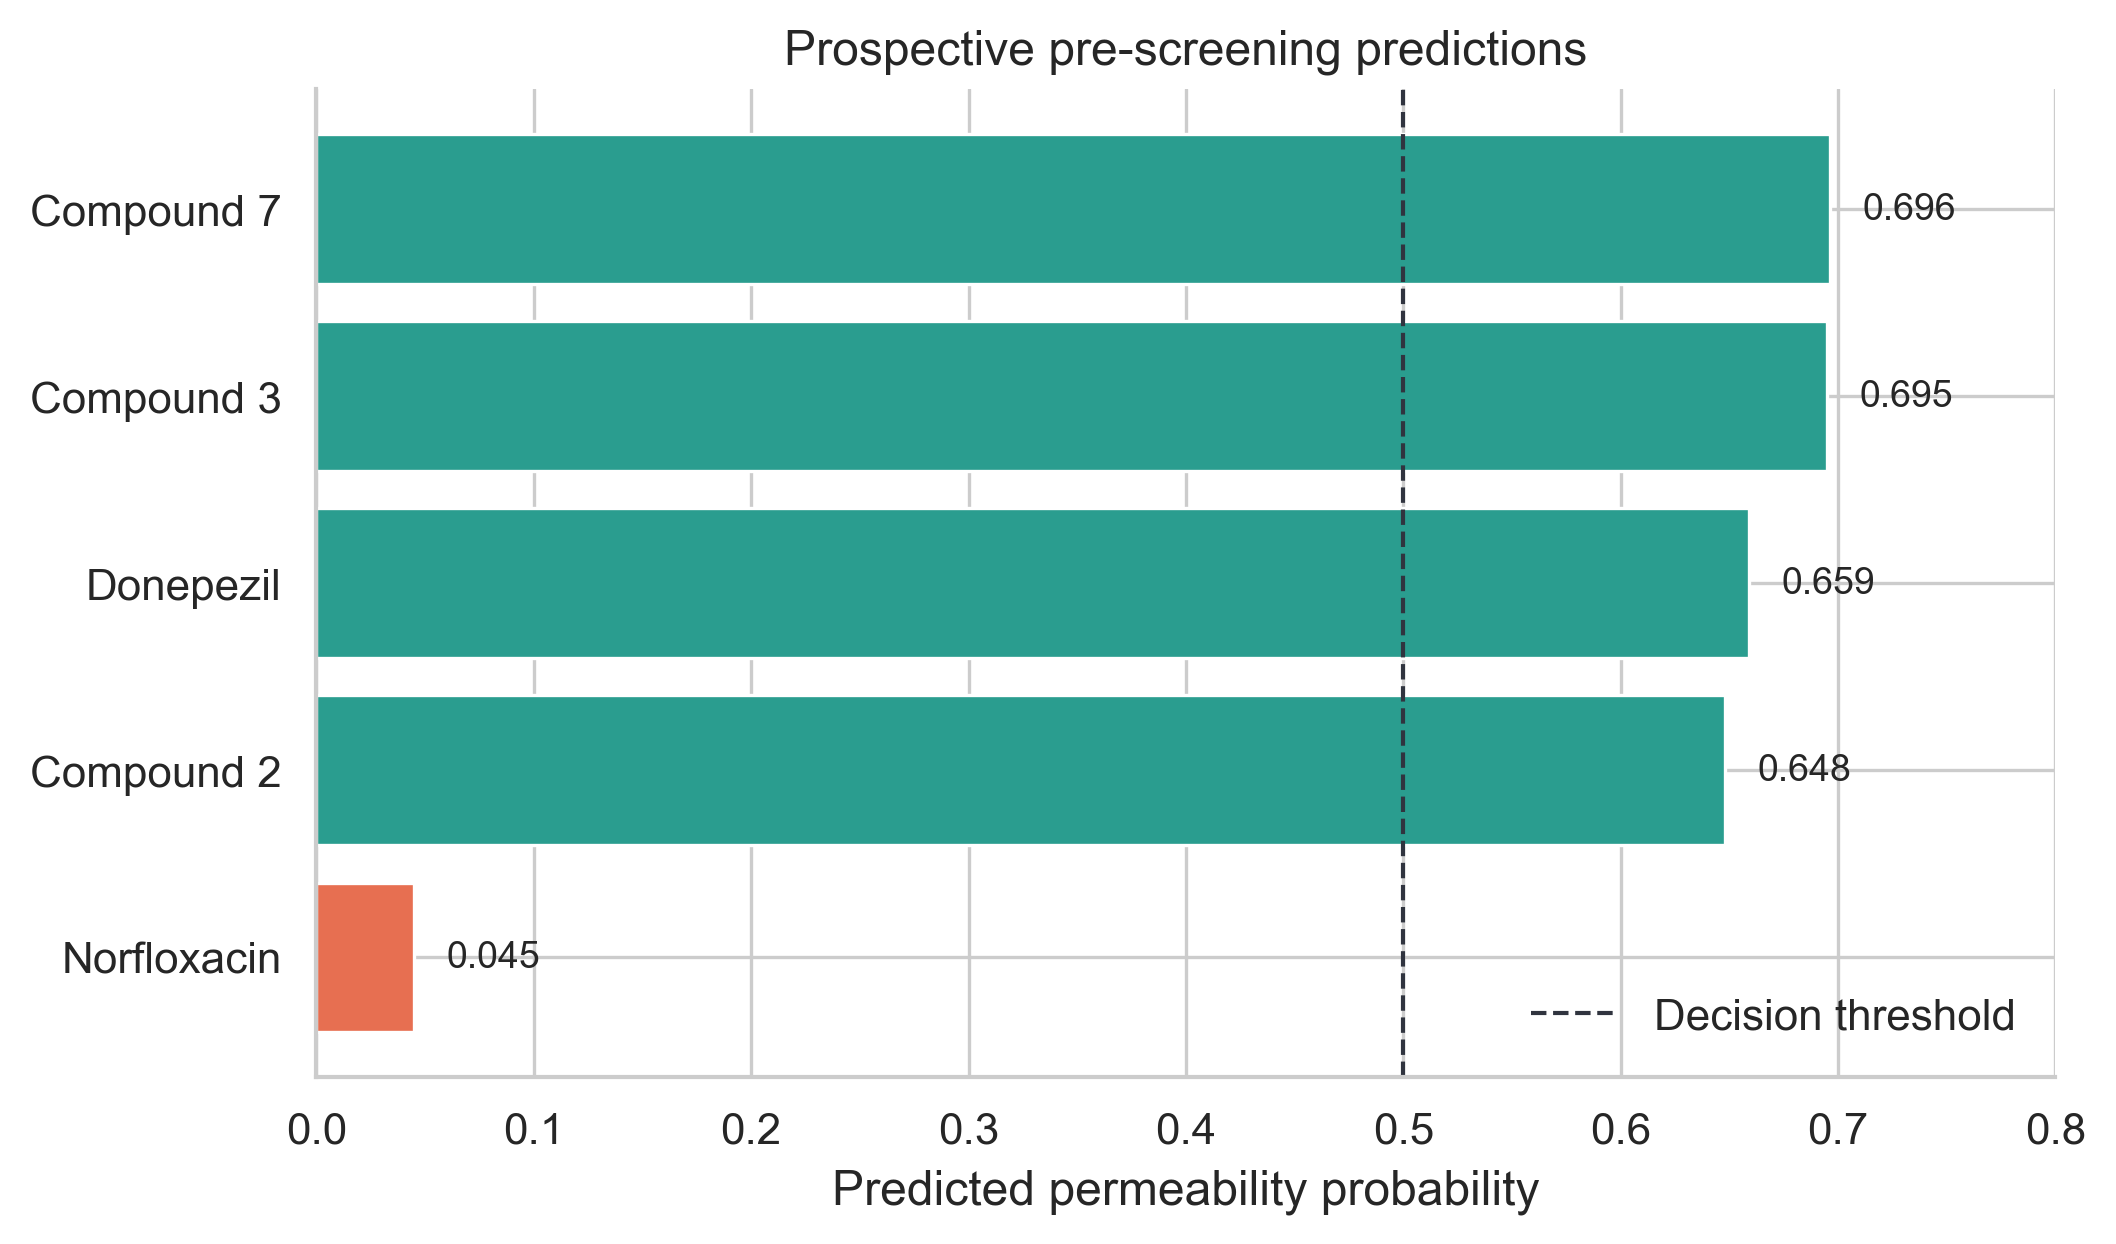
\includegraphics[width=0.78\textwidth]{figures/python_pre_screening_probabilities.png}
\caption{Python-generated bar plot of the five-molecule prospective pre-screening probabilities with thesis compound/control names.}
\label{fig:py_prescreening}
\end{figure}

\subsection{DrugBank virtual screening}
The DrugBank workflow was organized as a progressive filtering funnel. Starting from a source library of more than 10000 compounds, descriptor availability, model prediction and probability filtering retained 863 high-probability candidate entries with \(P(\mathrm{permeable}) \geq 0.60\). Applicability-domain analysis classified 850 candidates as inside the model domain and 13 as outside. Lipinski filtering identified 778 candidates as viable, 57 as non-viable and 28 as not evaluable; the strict final prioritized set contained 770 compounds that were both inside the applicability domain and Lipinski viable (Table~\ref{tab:py_drugbank_flow}). Table~\ref{tab:py_drugbank_summary} reports the numerical screening summary. The filtering funnel is visualized in Figure~\ref{fig:py_drugbank_flow}, the probability distribution in Figure~\ref{fig:py_drugbank_probability}, and the leverage-based applicability-domain profile in Figure~\ref{fig:py_drugbank_leverage}. The probability distribution ranged from 0.600 to 0.990, with a median of 0.760.

\begin{table}[H]
\centering
\caption{DrugBank virtual-screening funnel generated from the final candidate table.}
\label{tab:py_drugbank_flow}
\begin{tabular}{lrp{0.52\textwidth}}
\toprule
Stage & Compounds & Criterion \\
\midrule
Complete DrugBank source & >10000 & Starting screening library before descriptor availability and curation \\
High-probability candidates & 863 & Predicted permeable probability >= 0.60 \\
Inside applicability domain & 850 & Leverage h <= 0.0083 \\
Final prioritized candidates & 770 & Inside AD and Lipinski viable \\
\bottomrule
\end{tabular}
\end{table}

\begin{table}[H]
\centering
\caption{DrugBank screening summary generated from the final candidate table.}
\label{tab:py_drugbank_summary}
\begin{tabular}{lr}
\toprule
Metric & Value \\
\midrule
Final candidates & 863 \\
Inside applicability domain & 850 \\
Outside applicability domain & 13 \\
Lipinski viable & 778 \\
Lipinski non-viable & 57 \\
Not evaluable by Lipinski & 28 \\
Inside AD and Lipinski viable & 770 \\
Median probability & 0.760 \\
Maximum probability & 0.990 \\
\bottomrule
\end{tabular}
\end{table}

\begin{table}[H]
\centering
\caption{Top ten DrugBank candidates ranked by predicted PAMPA permeability probability with names recovered from the local DrugBank SDF metadata.}
\label{tab:py_top_drugbank}
\begin{tabular}{lp{0.28\textwidth}rrrrl}
\toprule
DrugBank ID & Generic name & Probability & Leverage & MW & LogP & Lipinski \\
\midrule
DB00404 & Alprazolam & 0.990 & 0.001 & 308.77 & 3.580 & Yes \\
DB03786 & 2-(3-Cyano-4-Isobutoxy-Phenyl)-4-Methyl-5-Thiazole-Carboxylic Acid & 0.980 & 0.001 & 316.38 & 3.720 & Yes \\
DB04854 & Febuxostat & 0.980 & 0.001 & 316.38 & 3.720 & Yes \\
DB03899 & 9-Butyl-8-(4-Methoxybenzyl)-9h-Purin-6-Amine & 0.970 & 0.001 & 311.39 & 2.810 & Yes \\
DB04920 & Clevidipine & 0.970 & 0.002 & 456.32 & 4.250 & Yes \\
DB00496 & Darifenacin & 0.960 & 0.001 & 426.56 & 3.960 & Yes \\
DB00561 & Doxapram & 0.960 & 0.002 & 378.52 & 3.170 & Yes \\
DB04715 & IMIDAZOPYRIDAZIN 1 & 0.960 & 0.001 & 306.37 & 3.420 & Yes \\
DB05838 & OPC-51803 & 0.960 & 0.001 & 454.01 & 5.380 & Yes \\
DB00656 & Trazodone & 0.953 & 0.002 & 371.87 & 2.360 & Yes \\
\bottomrule
\end{tabular}
\end{table}

\begin{table}[H]
\centering
\caption{DrugBank top-ten list reported in the thesis, cross-checked against local DrugBank SDF metadata and the current reproducible candidate table.}
\label{tab:py_drugbank_thesis_top10}
\begin{tabular}{lp{0.18\textwidth}p{0.24\textwidth}rrl}
\toprule
DrugBank ID & Thesis-reported name & SDF-verified name & Thesis probability & Current probability & Name audit \\
\midrule
DB06209 & Prasugrel & prasugrel & 0.980 & 0.946 & Match \\
DB01656 & Vatalanib & Roflumilast & 0.978 & 0.890 & Check ID/name \\
DB00838 & Clopidogrel & Clocortolone & 0.976 & 0.920 & Check ID/name \\
DB02300 & Calcipotriol & Calcipotriol & 0.970 & 0.920 & Match \\
DB00317 & Gefitinib & Gefitinib & 0.970 & 0.910 & Match \\
DB00401 & Propranolol & Nisoldipine & 0.970 & 0.940 & Check ID/name \\
DB00559 & Verapamil & Bosentan & 0.970 & 0.930 & Check ID/name \\
DB04967 & Lucanthone & Lucanthone & 0.970 & 0.930 & Match \\
DB04715 & Imidazopyridazine & IMIDAZOPYRIDAZIN 1 & 0.970 & 0.960 & Check ID/name \\
DB00269 & Chlorpromazine & Chlorotrianisene & 0.960 & 0.930 & Check ID/name \\
\bottomrule
\end{tabular}
\end{table}


The candidate ranking generated from the preserved CSV file is shown in Table~\ref{tab:py_top_drugbank}. For traceability with the thesis document, Table~\ref{tab:py_drugbank_thesis_top10} also reproduces the top-ten list reported in the thesis and cross-checks each DrugBank ID against the local DrugBank SDF metadata used by this repository. This audit is important because several thesis-reported generic names are not the generic names associated with the same DrugBank IDs in the local SDF; therefore, final pharmacological discussion should use the ID-name pairs verified from the screening source file.

\begin{figure}[H]
\centering
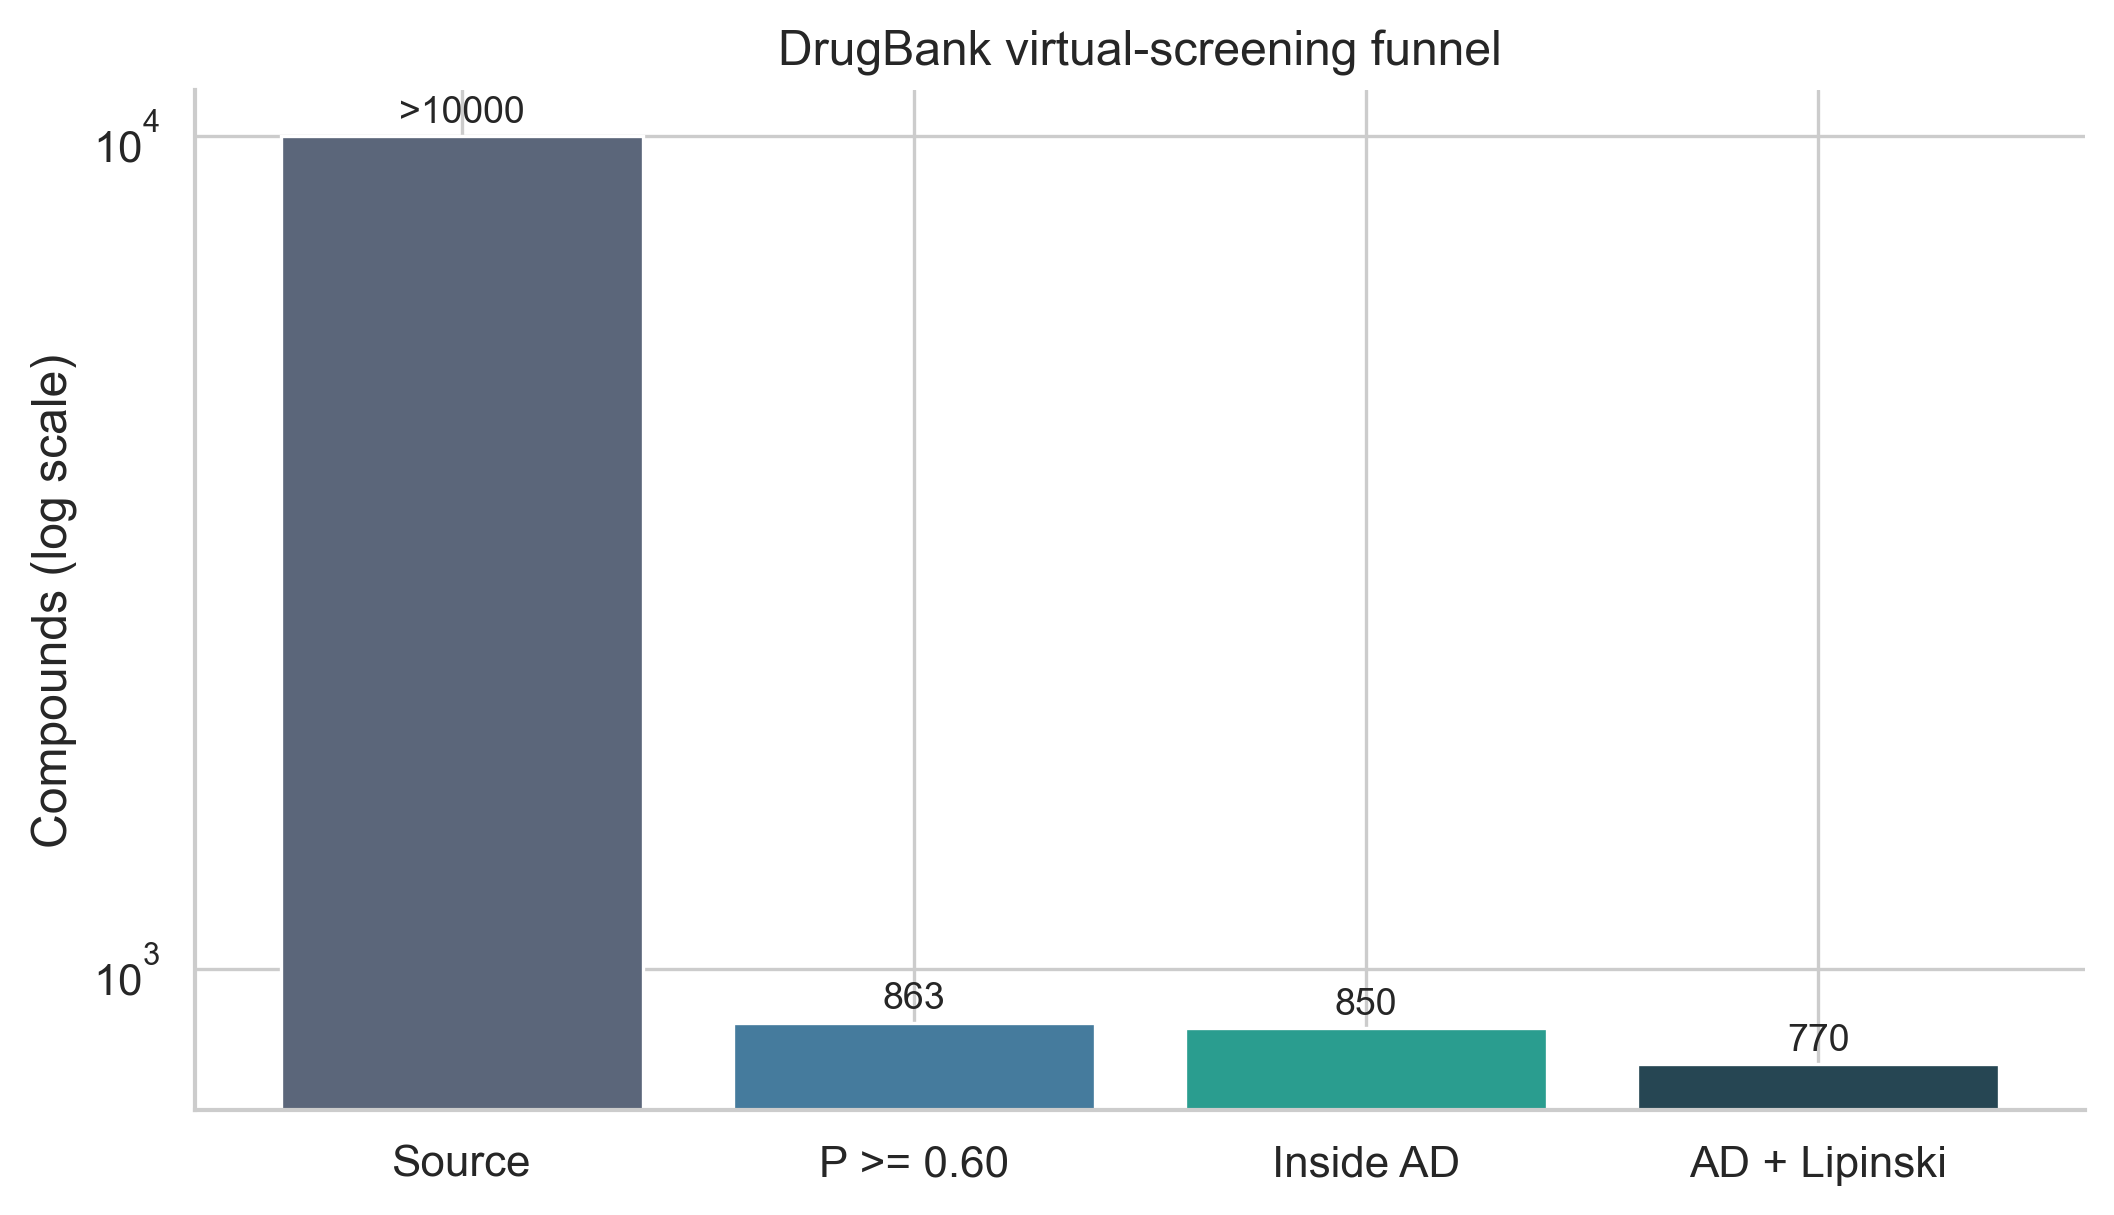
\includegraphics[width=0.78\textwidth]{figures/python_drugbank_filtering_flow.png}
\caption{Python-generated DrugBank virtual-screening funnel from the complete source library to the final prioritized candidates.}
\label{fig:py_drugbank_flow}
\end{figure}

\begin{figure}[H]
\centering
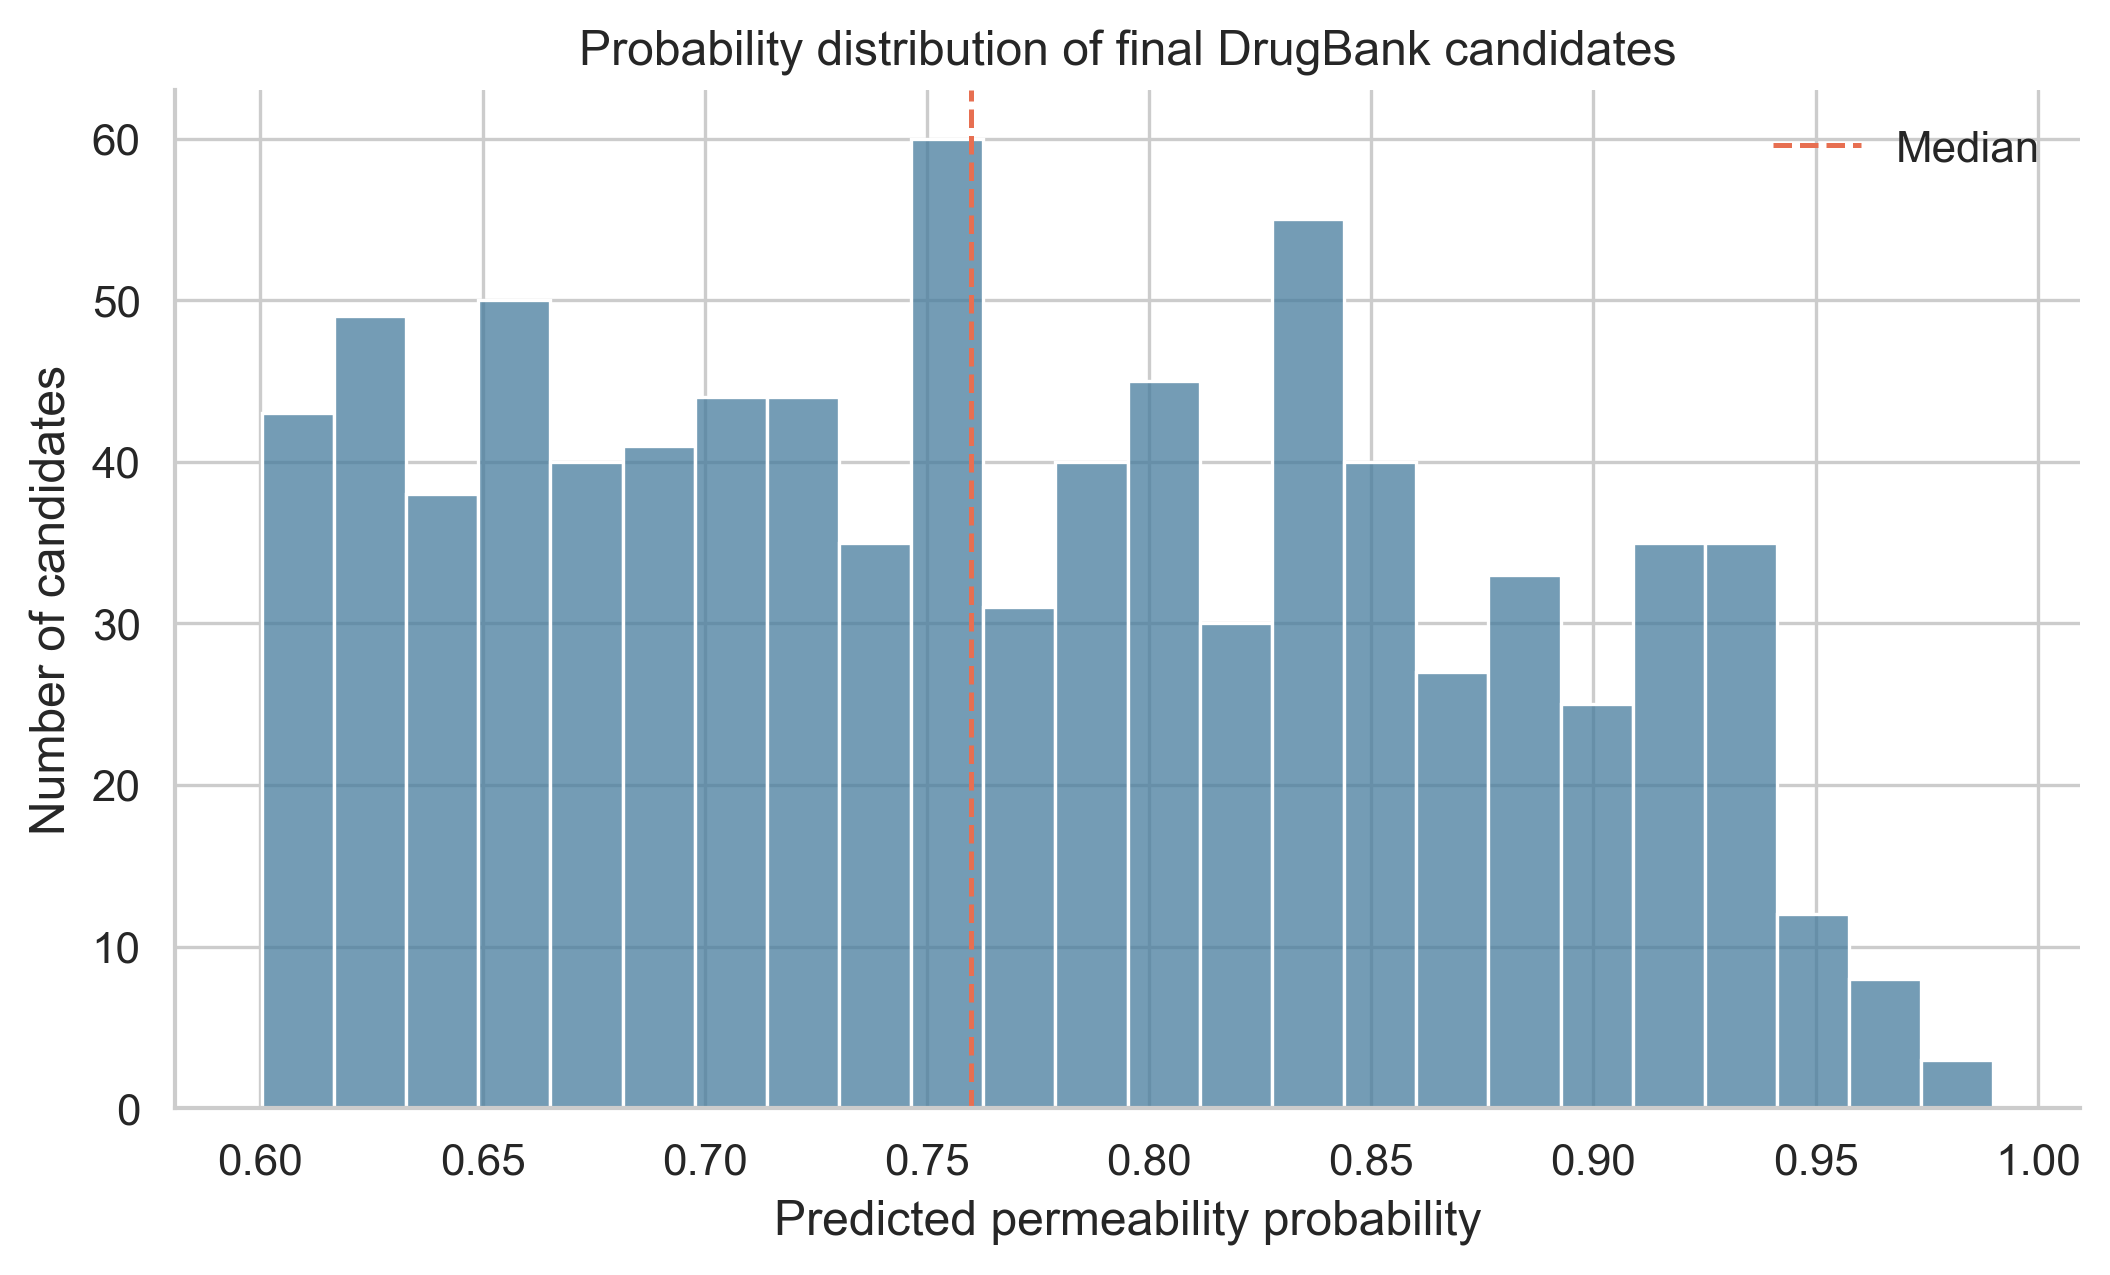
\includegraphics[width=0.78\textwidth]{figures/python_drugbank_probability_distribution.png}
\caption{Python-generated probability distribution for the final DrugBank candidate set.}
\label{fig:py_drugbank_probability}
\end{figure}

\begin{figure}[H]
\centering
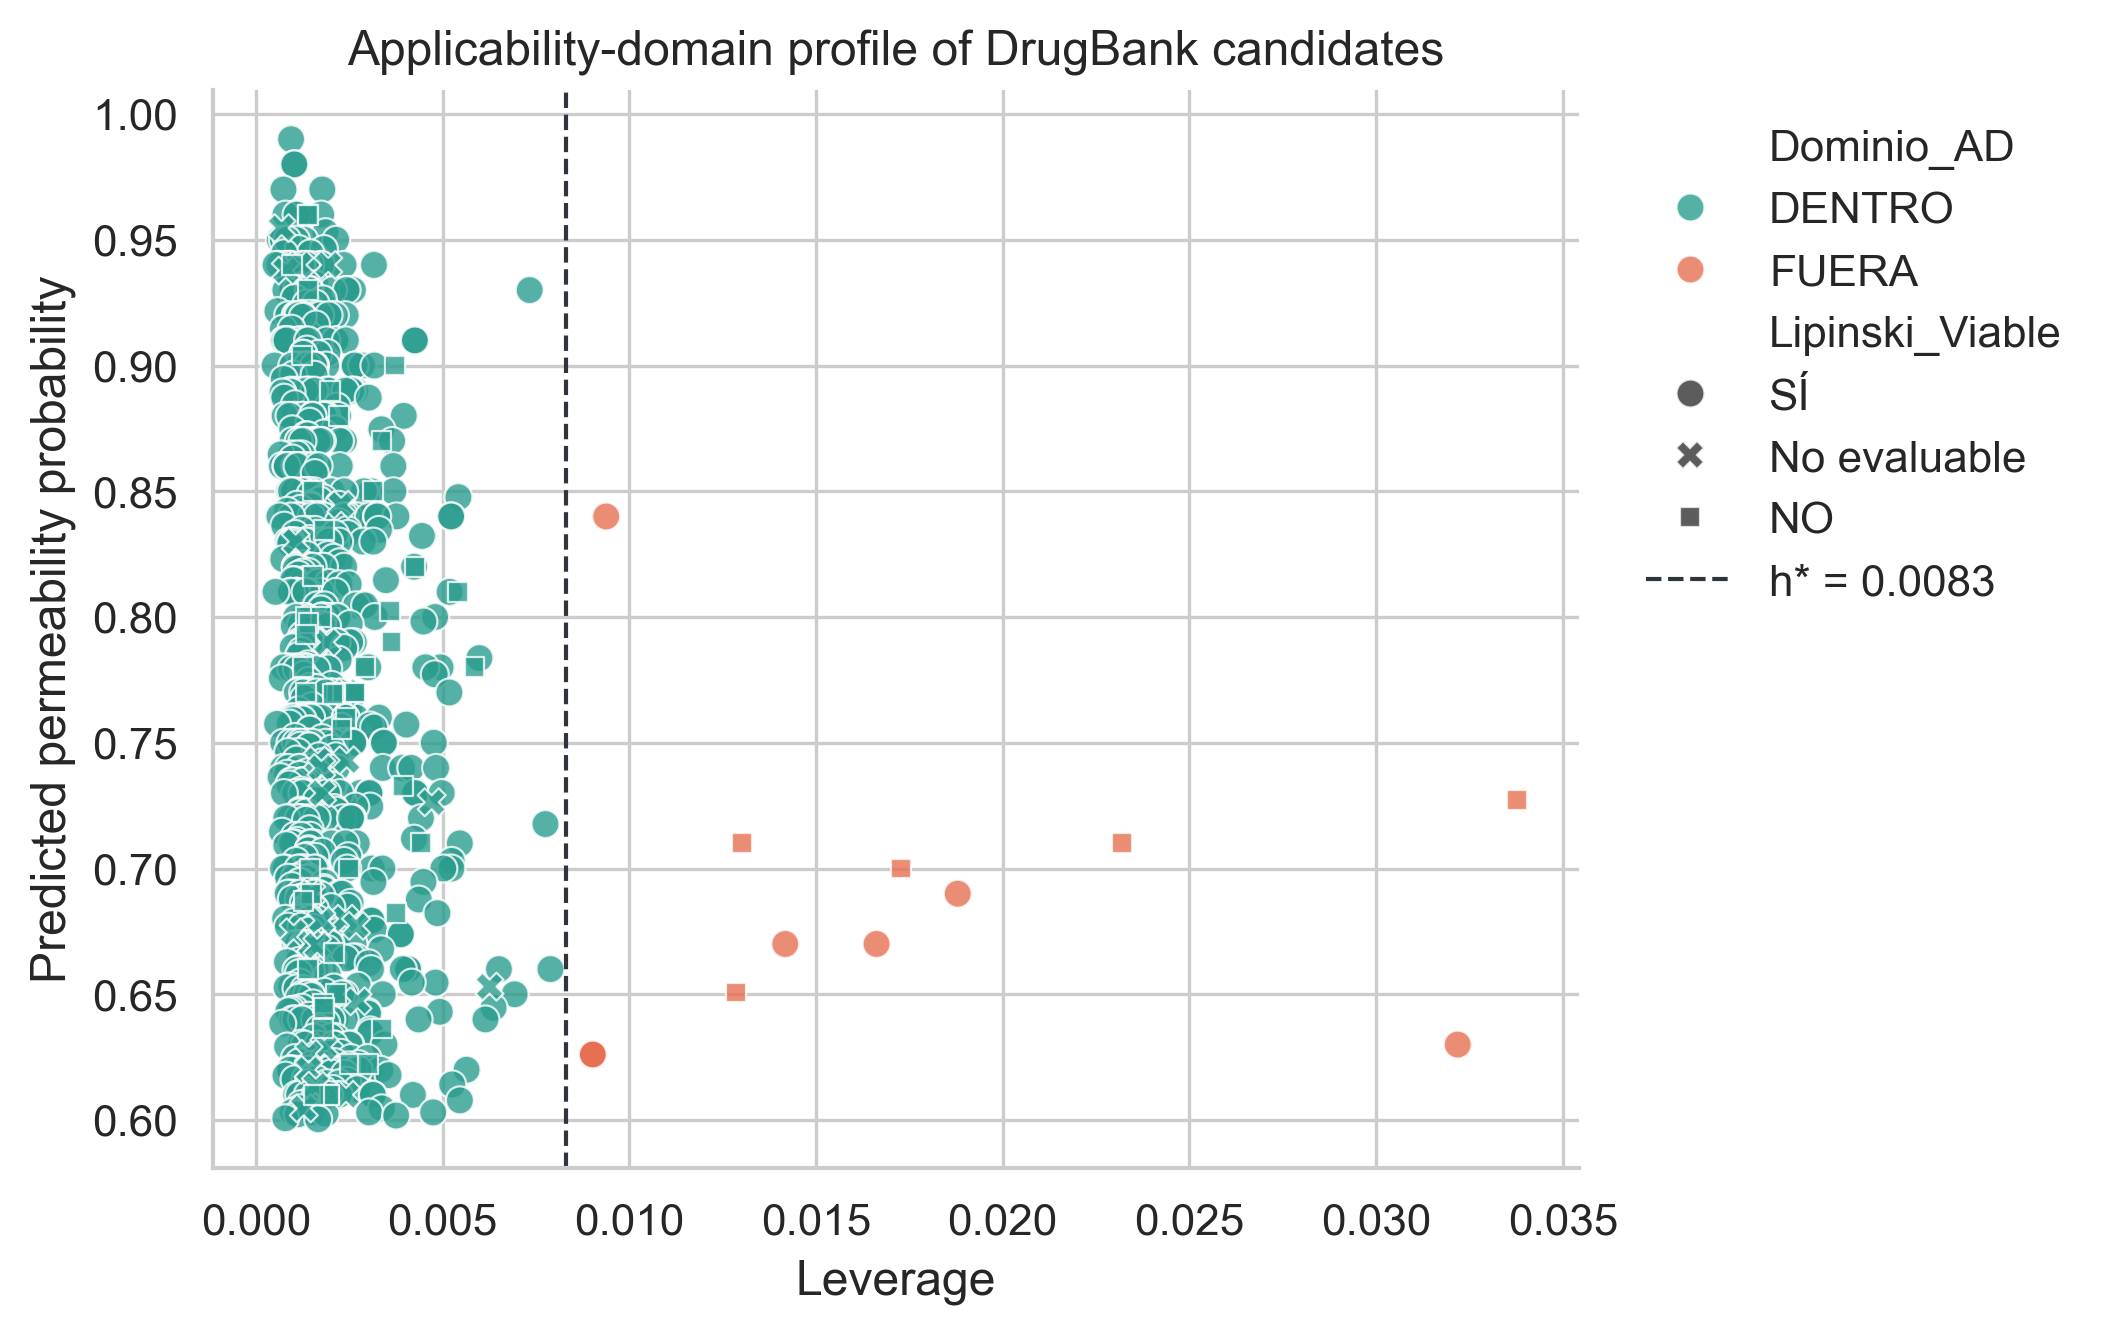
\includegraphics[width=0.86\textwidth]{figures/python_drugbank_leverage_probability.png}
\caption{Python-generated applicability-domain visualization for DrugBank candidates, showing leverage versus predicted permeability probability.}
\label{fig:py_drugbank_leverage}
\end{figure}

These results should be interpreted as a prioritization list rather than a definitive pharmacokinetic annotation, because PAMPA models describe passive permeability and do not account for active transport, metabolism, formulation effects or systemic exposure. The DrugBank names in the reproducible candidate table were recovered from the local DrugBank SDF metadata, keeping the reported IDs and chemical names tied to the same source file used in the screening workflow.

\section*{Python-generated supporting tables}
The tables in this section are generated by \texttt{manuscript/generate\_python\_assets.py} from the repository datasets and result files. Table~\ref{tab:py_dataset_composition} reproduces the curated dataset composition directly from the CSV files, Table~\ref{tab:py_cross_validation} reproduces the stored cross-validation metrics, and Table~\ref{tab:py_final_metrics} reproduces the final model metrics used in the main results section.

\begin{table}[H]
\centering
\caption{Dataset composition generated from the curated CSV files.}
\label{tab:py_dataset_composition}
\begin{tabular}{lrrrr}
\toprule
Dataset & Total & Permeable & Non-permeable & Permeable (\%) \\
\midrule
Training & 4357 & 2332 & 2025 & 53.5 \\
Internal test & 1090 & 583 & 507 & 53.5 \\
External validation & 486 & 443 & 43 & 91.2 \\
\bottomrule
\end{tabular}
\end{table}

\begin{table}[H]
\centering
\caption{Cross-validation metrics generated from the reproducible results.}
\label{tab:py_cross_validation}
\begin{tabular}{rrrrrr}
\toprule
K & Accuracy & Sensitivity & Specificity & AUC & F1-score \\
\midrule
5 & 0.738 & 0.729 & 0.746 & 0.823 & 0.735 \\
10 & 0.738 & 0.730 & 0.745 & 0.823 & 0.735 \\
\bottomrule
\end{tabular}
\end{table}

\input{tables/final_metrics.tex}

\section{Conclusions}
An interpretable Random Forest QSAR model was developed for passive intestinal permeability prediction using curated PAMPA data. The final 11-descriptor model was obtained through an explicit alvaDesc, EDA, RFE and WEKA consensus workflow and reproduced the thesis metrics, achieving strong performance in training and internal testing and high sensitivity in an independent external validation set. The descriptor panel is chemically meaningful and reflects the interplay between lipophilicity, polar surface contributions, polarizability, topology and structural fingerprints, with SHAP analysis providing an additional descriptor-level interpretation layer. The workflow also provides applicability-domain filtering and virtual screening output, enabling practical prioritization of compounds with favorable passive permeability profiles.

The model is most appropriate as an early-stage decision-support tool for passive permeability prioritization. Future work should expand the external non-permeable class, calibrate probability outputs, compare additional algorithms using nested validation and experimentally validate selected DrugBank candidates in standardized PAMPA assays.

\section*{Data and code availability}
The curated datasets, trained model, validation scripts, notebooks and screening outputs are available at \url{https://github.com/bvasquezp/Permeability-PAMPA-ML}. The final metrics can be reproduced with \texttt{python src/check\_final\_metrics.py}, and core file integrity can be checked with \texttt{python src/validate\_project.py}.

\section*{Author contributions}
Benjamin Andres Vasquez Perez: conceptualization, data curation, modeling, validation, visualization and writing original draft. Juan Alberto Castillo-Garit: supervision, methodology, scientific guidance and manuscript review. Author roles should be confirmed before submission.

\section*{Funding}
Funding information should be added before journal submission.

\section*{Conflicts of interest}
The authors declare no conflicts of interest. This statement should be confirmed before submission.

\section*{Acknowledgements}
The authors acknowledge Universidad Tecnologica Metropolitana and the thesis supervision process that supported the development of this work. Additional acknowledgements should be added before submission.

\bibliographystyle{unsrt}
\bibliography{references}

\end{document}
